%
% Modelo de trabalhos acadêmicos
% Documento principal
%
% Centro Federal de Educação Tecnológica de Minas Gerais - CEFET-MG
% Autor: Autor: Cristiano Fraga G. Nunes <cfgnunes@gmail.com>
%
%
% para melhor visualização deste código, altere as configurações
% de seu editor para largura da tabulação igual a 8
%

% TODO: conferir margens
% TODO: criar glossário
% TODO: criar índice remissivo

\documentclass[logo, oneside]{abnt-cefetmg}			% oneside = apenas frente da folha
%\documentclass[logo, openright, twoside]{abnt-cefetmg}		% openright = frente e verso (o capitulo começa sempre em páginas ípares)
%\documentclass[logo, oneside, trabalhos]{abnt-cefetmg}		% modelo de trabalhos comuns

% importações de pacotes
	\usepackage[alf, abnt-emphasize=bf, bibjustif, recuo=0cm, abnt-etal-cite=2, abnt-etal-list=0]{abntcite}	% fazer citações no padrão da ABNT
	
	\usepackage[font=small,labelfont=bf]{caption}
	\usepackage[algoruled]{algorithm2e}		% escrever algoritmos
	\usepackage{bookmark}					% cria menu de bookmarks
	\usepackage[brazil]{babel}				% escrita em português brasileiro
	\usepackage[utf8]{inputenc}				% acentuação direta
	\usepackage[T1]{fontenc}				% codificação da fonte em 8 bits
	\usepackage{graphicx}					% inserir figuras
	\usepackage{subfigure}						% posicionamento de figuras
	\usepackage{amsfonts, amssymb, amsmath, dsfont}	% fonte e simbolos matemáticos
	\usepackage{booktabs}					% comandos para tabelas
	\usepackage{verbatim}					% texto é interpretado no compilador como escrito no documento
	\usepackage{multirow, array}			% múltiplas linhas e colunas em tabelas
	\usepackage[bottom]{footmisc}			% mantem as notas de rodapé sempre na mesma posicao
	%\usepackage{acronym}					% produzir acrônimos
	%\usepackage{scalefnt}					% permite redimensionar tamanho da fonte
	%\usepackage{color, colortbl}			% comandos de cores
	%\usepackage{lscape}					% permite páginas em modo "paisagem"
	%\usepackage{breakurl} 					% permite quebra de linha em urls
	%\usepackage{ae,aecompl} 				% fontes de alta qualidade
	%\usepackage{picinpar} 					% dispor imagens em parágrafos
	%\usepackage{latexsym} 					% simbolos matematicos
	%\usepackage{upgreek} 					% fonte letras gregas
	%\usepackage{dsfont} 					% fonte matematica
	%\usepackage{type1ec} 					% fonte Times
	%\usepackage{pxfonts} 					% fonte
	%\usepackage{palatino} 					% fonte palatino
	%\usepackage{psfrag}					% símbolos latex em figuras eps
	%\usepackage{subeqnarray} 				% sub enumeração de equações
	%\usepackage{bibentry} 					% uso de bibtex inline
	%\usepackage{makeidx} 					% produzir índice remissivo (glossario)
	%\usepackage{multind} 					% produzir índices múltiplos 
	\usepackage{fancyhdr} 					% cabeçalhos
	\usepackage{pslatex}					% Fonte times 
%	\usepackage{cite}
% inclui o prêambulo do documento
	%
% Documento: Preâmbulo
%

% nome da instituicao
\instituicao{Centro Federal de Educação Tecnológica de Minas Gerais}

% nome do programa
\programa{Curso de Engenharia de Computação}

% nome do departamento
\departamento{Departamento de Computação}

% área
%\area{Área de concentração}

% Dissertação, Tese, Monografia
\documento{Monografia}

% Mestre, Doutor, Engenheiro
\titulacao{Engenheiro de Computação}

% titulo do trabalho em portugues
\titulo{Comparação de algoritmos paralelos de ordenação em MapReduce}

% subtitulo do trabalho em portugues, se houver
%\subtitulo{Subtítulo do Trabalho}

% titulo do trabalho em ingles
\title{Performance evaluation of paralell sorting algorithms in MapReduce}

% autor do trabalho
\autor{Mariane Raquel Silva Gonçalves}
%\autordois{Nome do segundo autor}

% palavras-chave do trabalho
\palavraschave{Palavra-chave 1, Palavra-chave 2, ...}

% palavras-chave do trabalho em ingles
\keywords{Keyword 1, Keyword 2, ...}

\comentario{\DOCdocumentodata{} apresentada ao \DOCprogramadata{} do \ABNTinstituicaodata{}, como requisito parcial para obtenção do grau de \DOCtitulacaodata{}.}

% nome do orientador do trabalho
%\orientador{Nome do orientador}
\orientador[Orientadora:]{Profª. Drª. Cristina Duarte Murta}

% nome do co-orientador do trabalho, caso exista
%\coorientador{Nome do co-orientador}
%\coorientador[Co-orientadora:]{Nome da co-orientadora}

% no caso de 2 co-orientadores, usar esta sintaxe
%\coorientador[Co-orientadores:]{Nome do co-orientadorA}
%\coorientadorb{Nome do co-orientadorB}

% local
\local{Belo Horizonte}

% data
\data{2013}

% texto da folha de apresentação
\textoaprovacao{\DOCdocumentodata{} julgada e aprovada, para a obtenção do grau de \DOCtitulacaodata{} no \DOCprogramadata{}.}

% data da folha de aprovação
\localdia{Belo Horizonte, 1 de abril de 2013}

% nome da primeira pessoa a assinar a folha de apresentação
\primeiroassina{Professor A \\ Instituição}

% nome da segunda pessoa (se houver) a assinar a folha de apresentação
\segundoassina{Professor B \\ Instituição}

% nome da terceira pessoa (se houver) a assinar a folha de apresentação
%\terceiroassina{Professor C \\ Instituição}

% nome da quarta pessoa (se houver) a assinar a folha de apresentação
%\quartoassina{Professor D \\ Instituição}




% hifenização de palavras desconhecidas
%	\hyphenation{
%		Na-ra-ya-nan
%		qua-dros-cha-ves
%		Bras-nett
%		Kat-sa-gge-los
%	}

% define as cores dos links e informações do pdf
\hypersetup{
	colorlinks,
	linkcolor=black,
	citecolor=black,
	filecolor=black,
	urlcolor=black,
	breaklinks=true,
	pdftitle={\ABNTtitulodata},
	pdfauthor={\ABNTautordata},
	pdfsubject={\ABNTcomentariodata},
	pdfkeywords={\DOCpalavraschavedata}
}

% pode-se utilizar os comandos abaixo para realizar ajustes das margens se necessário
\usepackage{geometry}
\geometry{left=3.0cm, right=2.5cm, top=3.0cm, bottom=3cm} 

\usepackage{estilo}

% início do documento
\begin{document}


%% elementos pré textuais
%	\capa												% Capa
%	\folhaderosto										% Folha de rosto
%    	\folhadeaprovacao									% Folha de aprovação
%	%%
% Documento: Dedicatória
%

\begin{dedicatoria}
Espaço reservado para dedicatória.
Inserir seu texto aqui...
\end{dedicatoria}

			% Dedicatória
%	% Agradecimentos - é so para as pessoas que contribuiram relevantemente
% para a elaboração do trabalho
\pretextualchapter{Agradecimentos}

\begin{minipage}{\textwidth}
    Agradeço aos meus pais, pelo amor incondicional. \\
    Aos meus professores, pelos conhecimentos adquiridos. \\
     E finalmente aos colegas de curso pela convivência e trocas de experiências.
\end{minipage}

		% Agradecimentos
%	%%
% Documento: Epígrafe
%

\begin{epigrafe}

\textit{``O fator decisivo para vencer o maior obstáculo é, invariavelmente, ultrapassar o obstáculo anterior.'' (Henry Ford)}

\end{epigrafe}
			% Epígrafe
%	%
% Documento: Resumo (Português)
%

\begin{resumo}
Inserir seu texto aqui... (máximo de 500 palavras)
\end{resumo}
			% Resumo na língua vernácula
%	%
% Documento: Resumo (Inglês)
%

\begin{abstract}
Inserir seu texto aqui... (máximo de 500 palavras)
\end{abstract}
			% Resumo em língua estrangeira
%	\listadefiguras										% Lista de figuras
%	%\listadequadros										% Lista de quadros
%	\listadegraficos 									% Lista de gráficos
%	\listadetabelas										% Lista de tabelas
%	%\listadesiglas										% Lista de abreviaturas e siglas
%	%\listadesimbolos 	 								% Lista de símbolos
	\sumario												% Sumário

% elementos textuais
	%
% Documento: Introdução
%

\chapter{Introdução}\label{chap:introducao}

Esse capítulo apresenta o contexto da computação que torna relevante o estudo e a comparação de algoritmos de ordenação paralela no modelo MapReduce, sobretudo na implementação Hadoop; o crescimento de dados que contribuiu para a necessidade de mudança da computação sequencial para a computação paralela e a importância dos algoritmos de ordenação, utilizados em diversas aplicações. Adicionalmente, busca delimitar o tema a ser tratado, os objetivos do trabalho e sua estrutura de capítulos.  


\section{Caracterização do Problema}
\label{sec:caracProblema}

Na última década, a quantidade de dados  disponível na web, gerada e processada por empresas e sistemas computacionais, aumentou várias ordens de grandeza, fazendo do processamento dos dados um desafio para a computação sequencial. Como resultado, torna-se crucial substituir a computação tradicional pela computação distribuída eficiente \cite{Lin:2010}. A mudança no modelo de programação sequencial para paralelo é um fato inevitável e ocorre gradualmente, desde que a indústria declarou que seu futuro está em computação paralela \cite{Asanovic:2009}.

A ordenação é um dos problemas fundamentais da ciência da computação e um dos problemas algorítmicos mais estudados. Suas aplicações vão desde sistemas de banco de dados à computação gráfica, além de muitos outros algoritmos que podem ser descritos em termos de ordenação \cite{Satish:2009,Amato:1996}.  Muitas aplicações dependem de ordenações eficientes como base para seu próprio desempenho, que podem ser desenvolvidas através de rotinas eficientes de ordenação em arquiteturas paralelas e distribuídas. 
O uso crescente de computação paralela em sistemas computacionais gera a necessidade de algoritmos de ordenação inovadores, desenvolvidos para dar suporte a essas aplicações. 
 

Com a constante evolução das arquiteturas de computadores há uma necessidade contínua de explorar técnicas de ordenação em arquiteturas emergentes. 
Nesse sentido, são desenvolvidos diferentes modelos de programação paralela para ambientes \textit{multicore} e distribuído, como o MapReduce. O MapReduce é um modelo de programação paralela desenvolvido pela Google para processamento de grandes volumes de dados distribuídos em \textit{clusters} \cite{Dean:2008}. Esse modelo propõe simplificar a computação paralela, escondendo  do desenvolvedor os detalhes da paralelização e utilizando duas funções principais - Map e Reduce.
Uma das implementações mais conhecidas e utilizadas do modelo é o Hadoop \cite{White:2009}, ferramenta de código aberto, desenvolvida por Doug Cutting em 2005 e apoiada pela Yahoo!. 



O trabalho proposto por %\citeonline{Paula:2011} 
Pinhão (2011) apresentou uma avaliação da escalabilidade 
%- habilidade de um sistema manipular uma porção crescente de trabalho de forma uniforme - 
de algoritmos de ordenação paralela no modelo MapReduce. Para tal, foi desenvolvido o algoritmo de Ordenação por Amostragem, no ambiente Hadoop, e seu desempenho foi avaliado em relação à quantidade de dados de entrada e ao número de máquinas utilizadas. 

Considerando esse contexto, o presente trabalho segue o tema e busca continuar o estudo com a implementação e análise de escalabilidade, em relação à quantidade de dados a ser ordenada e de número de máquinas utilizadas, do algoritmo \textit{Quicksort} Paralelo, no modelo MapReduce e ambiente Hadoop. Outro ponto é a comparação do desempenho dos dois algoritmos - Ordenação por Amostragem e \textit{Quicksort} Paralelo - em diferentes cenários.


\section{Motivação}
\label{sec:motivacao}


% 1. crescimento dos dados requer mais poder computacional

O volume de dados que é produzido e tratado diariamente em indústrias, empresas e até mesmo em âmbito pessoal teve um rápido crescimento nos últimos anos, tornando o desenvolvimento de soluções capazes de lidar com tais volumes de dados uma das grandes preocupações atuais. Estima-se que dados não estruturados são a maior porção e a de mais rápido crescimento dentro das empresas. 
%, tendo em vista a quantidade de dados processados , e o  desse volume de dados.
Não é fácil medir o volume total de dados armazenados digitalmente, mas uma estimativa da \textit{International Data Corporation} (IDC) calculou o tamanho do universo digital em 0,18 zettabytes em 2006, prevendo um crescimento de dez vezes até 2011, chegando a 1,8 zettabytes \cite{Gantz:2008}.
Em 2008, o Facebook armazenava aproximadamente 10 bilhões de fotos, que ocupavam mais de um petabyte. \textit{The Internet Archive} armazenava aproximadamente 2 petabytes de dados, com acréscimo de 20 terabytes por mês e a Bolsa de Valores de Nova Iorque gerava cerca de um terabyte de novos dados comerciais por dia
\cite{White:2009}. %, o que torna o processamento de tal volume de dados muitas vezes inviável.

%2. mais poder computacional pode ser conseguido com a) clock  e b) paralelismo

Mesmo para os computadores atuais, é um desafio conseguir lidar com quantidades de dados tão grandes. É preciso buscar soluções escaláveis, que apresentem bom desempenho mesmo com aumento significativo no número de recursos e na carga de trabalho. 
%3. a indústria sabe que agora só é possível trabalhar o paralelismo
Nos últimos 40 anos, o aumento do poder computacional deveu-se, largamente, ao aumento da capacidade do hardware. Atualmente, o limite físico da velocidade do processador foi alcançado e arquitetos sabem que o aumento no desempenho só pode ser alcançado com o uso de computação paralela. Com isso, a indústria têm recorrido cada vez mais a arquiteturas paralelas para continuar a fazer progressos \cite{Manferdelli:2008}. 

As tendências atuais estão redirecionando o foco da computação, do tradicional modelo de processamento científico para o processamento de grandes volumes de dados.
Nesse sentido, arquiteturas paralelas, como as de memória distribuída, estão cada vez mais frequentes, suprindo a necessidade de uma computação distribuída eficiente, que forneça alto desempenho no processamento de dados \cite{Bryant:2011}.
%substituir a computação sequencial 
%.por, cujo foco sejam os dados e . 


% 4. computação paralela é dificil

As técnicas tradicionais de programação paralela - como passagem de mensagens e memória compartilhada - em geral são complexas e de difícil entendimento para grande parte dos desenvolvedores. Em tais modelos é preciso gerenciar localidades temporais e espaciais; lidar explicitamente com concorrência, criando e sincronizando \textit{threads} através de mensagens e semáforos. Dessa forma, não é uma tarefa simples escrever códigos paralelos corretos e escaláveis para algoritmos não triviais \cite{Breshears:2009}.

% 5. com o map reduce, é possível ordenar de forma rápida e fácil

O MapReduce surgiu como uma alternativa aos modelos tradicionais, com o objetivo de simplificar a computação paralela. 
%O maior benefício desse modelo é a simplicidade. 
O foco do programador é a descrição funcional do algoritmo e não as formas de paralelização. Nos últimos anos o modelo têm se estabelecido como uma das plataformas de computação paralela mais utilizada no processamento de terabytes e petabytes de dados \cite{Ranger:2007}.
%É um caminho natural para o processamento de dados em larga escala o uso de \textit{clusters}. 
MapReduce e sua implementação código aberto Hadoop oferecem  uma alternativa economicamente atraente através de uma plataforma eficiente de computação distribuída, capaz de lidar com grandes volumes de dados e mineração de petabytes de informações não estruturadas \cite{Cherkasova:2011}.

% 6. com o crescimento dos dados no mundo, ordenar está cada vez mais complexo 
Mesmo com o grande processamento  empregado em interfaces gráficas, visualização e jogos, a ordenação continua a ser uma parte considerável da computação e estima-se que seja responsável por aproximadamente 80\% dos ciclos de processamento\cite{Ranger:2007}. O uso de algoritmos paralelos de ordenação em tais aplicações melhora o tempo de execução do algoritmo e torna viável o processamento de grande quantidades de dados.


\section{Justificativa}
\label{sec:justificativa}

Os algoritmos paralelos para ordenação têm sido objeto de estudo desde o princípio da computação paralela, uma vez que a  ordenação é um dos problemas fundamentais da ciência da computação.
Um grande número de aplicações possui uma fase de computação intensa, na qual uma lista de elementos deve ser ordenada com base em algum de seus atributos. Um exemplo é o algoritmo de Page Rank \cite{Page:1999} da Google: as páginas de resultado de uma consulta são classificadas de acordo com sua relevância, e depois precisam ser ordenadas de maneira eficiente \cite{Kale:2010}. 
 

%Presenting the results from database queries, compiling a list of business investments with associated risk-reward measures, and figuring the company payroll are all operations that require sorting.  Every time you get a list of URLs from a search engine, the results have been sorted, typically by some measure of relevance to your original query.

%\textcolor{red}{Os algoritmos ótimos existentes em arquitetura sequencial, como Quicksort e Heapsort necessitam de um tempo mínimo \textit{(n log n)} para ordenar uma sequência de \textit{n} elementos \cite{Aho:1974}}.

% 7. a ordenação paralela pode melhorar essa tarefa

Na ordenação paralela, fatores como movimentação de dados, balanço de carga, latência de comunicação e distribuição inicial das chaves são considerados ingredientes chave para o bom desempenho, e variam de acordo com o algoritmo escolhido como solução \cite{Kale:2010}.  No exemplo do Page Rank, o número de páginas a serem ordenadas é enorme, e elas são recolhidas de diversos servidores da Google, assim é uma questão fundamental escolher algoritmo paralelo com o melhor desempenho dentre as soluções possíveis.
% 8. mas algoritmos paralelos são muito dependentes de ambiente e distribuição inicial, portanto é importante avaliar o desempenho desses algoritmos
Dado o grande número de algoritmos de ordenação paralela e grande variedade de arquiteturas paralelas, é uma tarefa difícil escolher um algoritmo genérico para diferentes máquinas e instâncias do problema.

 Além disso, não existe um modelo teórico conhecido que possa ser aplicado para prever com precisão o desempenho de um algoritmo em arquiteturas diferentes \cite{Amato:1996}.
Assim, estudos experimentais assumem uma crescente importância para a avaliação e seleção de algoritmos apropriados para ambientes paralelos. É preciso que estudos sejam realizados para que determinado algoritmo possa ser recomendado em certa arquitetura com alto grau de confiança.




\section{Objetivos}
\label{sec:objetivos}

\subsection{Objetivo Geral}
\label{subsec:objetivoGeral}

Este projeto busca continuar o estudo sobre ordenação paralela desenvolvido por Pinhão (2011), com a análise de desempenho dos algoritmos de ordenação Ordenação por Amostragem e \textit{Quicksort}. No citado trabalho, foi feito um estudo sobre a computação paralela e algoritmos de ordenação no modelo MapReduce, com a implementação do algoritmo de Ordenação por Amostragem em ambiente Hadoop. 
No presente trabalho busca-se comparar os algoritmos Ordenação por Amostragem e \textit{Quicksort} Paralelo em relação à quantidade de dados a serem ordenados, variabilidade dos dados de entrada e número máquinas utilizadas. 


\subsection{Objetivos Específicos}
\label{subsec:objetivosEspecificos}

Desse modo, os objetivos deste trabalho são:

\begin{packed_enum}
\item Estudar a programação paralela aplicada a algoritmos de ordenação;
\item Implementar o algoritmo de ordenação  \textit{Quicksort} no modelo MapReduce, com o \textit{framework} Hadoop;
\item Comparar as implementações dos algoritmos de ordenação paralela: Ordenação por Amostragem e \textit{Quicksort} Paralelo em termos de desempenho.
\end{packed_enum}

\section{Organização do Texto}
\label{sec:organizacaoTexto}

Esse projeto está organizado em sete capítulos. O próximo capítulo apresenta o referencial teórico para o desenvolvimento do trabalho, com conceitos de computação paralela  e do modelo MapReduce. O Capítulo \ref{cap:ordenacao} complementa o referencial teórico e apresenta os conceitos da ordenação de dados e ordenação paralela. 
O Capítulo \ref{cap:desenvolvimento} descreve a metodologia de pesquisa, indicando os passos seguidos durante o desenvolvimento. Os resultados preliminares obtidos até a entrega do projeto são apresentados no Capítulo \ref{cap:resultados}. As conclusões e os próximos passos para a finalização do projeto estão no Capítulo \ref{cap:conclusoes}.
			% Introdução
	\chapter{Computação Paralela}
\label{cap:referencial}

Esse capítulo aborda os principais conceitos envolvidos no trabalho,  como computação paralela, o modelo MapReduce e sua implementação de código aberto Hadoop.


\section{Definições}

A computação paralela constitui-se de uma coleção de elementos de processamento que se comunicam e cooperam entre si e com isso resolvem um problema de maneira mais rápida \cite{Almasi:1994}. Mesmo com o avanço tecnológico das últimas décadas, as arquiteturas de Von Neumann demostram deficiências quando utilizadas por aplicações que necessitam de grande poder computacional. Essa deficiência impulsionou a utilização da computação paralela, com o objetivo de aumentar a capacidade de processamento das máquinas.

No estudo de computação paralela, é importante diferenciar os conceitos de paralelismo e concorrência, pois ambos tratam de programação e execução de tarefas em múltiplos fluxos, implementados com o objetivo de resolver um único problema. Concorrência consiste em diferentes tarefas serem executadas ao mesmo tempo, de forma a produzir um resultado particular mais rapidamente. Isso não implica necessariamente na existência de vários elementos de processamento; a concorrência pode ocorrer tanto com um único processador quanto com múltiplos processadores. 
Por outro lado, o paralelismo exige a execução de diversas tarefas simultaneamente, com a necessidade de vários elementos de processamento. 
Se há apenas um elemento de processamento não há paralelismo, pois apenas uma tarefa será executada a cada instante, mas pode haver concorrência, pois o processador pode ser compartilhado pelas tarefas em execução \cite{Breshears:2009}.

% Desafios da computação paralela e medidas de desempenho
Comparada à computação sequencial, a computação paralela apresenta alto desempenho e soluções mais naturais para problemas intrinsecamente paralelos, contudo sua utilização também inclui desvantagens. O desenvolvimento de soluções paralelas apresenta maior dificuldade na programação, pois há mais detalhes e diversidades na implementação, uma vez que um programa paralelo envolve múltiplos fluxos de execução simultâneos e é preciso coordenar todos os fluxos para completar uma dada computação. Além disso há a necessidade de sincronismo e de balanceamento de cargas \cite{Rauber:2010}. 	Assim, o desenvolvimento de software paralelo introduz três principais desafios: assegurar confiabilidade de software, minimizar o tempo de desenvolvimento e conquistar bom desempenho na aplicação \cite{Leiserson:2008}.

Manter a confiabilidade do sistema é essencial, pois ao se introduzir paralelismo à aplicação, ela se torna vulnerável às condições de corrida e dependendo da ordem de execução das tarefas pode se comportar de forma diferente. Mesmo se nenhuma alteração for feita no hardware ou nos arquivos de entrada, execuções consecutivas da mesma aplicação podem produzir resultados diferentes. Lidar com situações como essa é particularmente desafiante, pois tais erros são assíncronos e ocorrem eventualmente, o que torna difícil evitá-los e encontrá-los durante testes.

Outro desafio é minimizar o tempo de desenvolvimento, já que muitas vezes o desenvolvimento paralelo é mais complexo que o sequencial e demanda, do desenvolvedor, conhecimento prévio de paralelismo. Em geral, é preciso maior tempo para escrever o código e a depuração é mais trabalhosa, 	diversos testes devem ser feitos no sistema, o que pode dispender maior tempo.

O bom desempenho da aplicação é um dos objetivos centrais da paralelização, mas pode ser comprometido por comunicação excessiva ou balanceamento irregular de carga. O balanceamento de carga busca atingir um aproveitamento ótimo dos recursos do sistema, alocando tarefas de forma a obter o mesmo nível de esforço em todos os processadores.  A comunicação e sincronização de tarefas devem ser minimizadas pelo desenvolvedor, pois são tipicamente as maiores barreiras para se atingir grande desempenho em programas paralelos.
Após o desenvolvimento de uma aplicação paralela é importante avaliar se os tempos de execução paralelos são menores que os sequenciais e quão menores são esses tempos, através de indicadores de desempenho. Para avaliar o desempenho de algoritmos paralelos as principais métricas são o \textit{speedup}, a eficiência e a lei de Amdahl.

O \textit{speedup} (S$_p$) é uma métrica que informa quão mais rápida é a aplicação paralela, em comparação com sua versão sequencial. Para isso, determina a relação existente entre o tempo gasto para executar um algoritmo  em um único processador ($T_{sequencial}$) e o tempo gasto para executá-lo em $p$ processadores (T$_{paralelo}$): 
\[ S_p = \frac{T_{sequencial}}{T_{paralelo}} \]	
Em uma situação ideal o \textit{speedup} é igual a $p$, o que indicaria que o aumento da capacidade de processamento é diretamente proporcional ao número de processadores. 
Contudo,  o \textit{speedup} é diretamente afetado por fatores como comunicação entre processos, granulosidades inadequadas e partes não paralelizáveis de programas.


 A eficiência (E$_p$) é outro parâmetro utilizado para medir o desempenho na computação paralela.  Ela relaciona o \textit{speedup} ao número de processadores, identificando a taxa de utilização do processador. Pode ser calculada por: \[ E_p = \frac{S_p}{p} \]
Enquanto o \textit{speedup} relaciona tempos de execução, a eficiência avalia o quão bem estão sendo utilizados os recursos do sistema. Em uma paralelização ideal a eficiência tem valor 1, significando que os processadores têm utilização total.
		
A Lei de Amdahl é outra importante métrica, que fornece um limite superior para o valor do \textit{speedup} que pode ser atingido em um sistema. Para aplicar a lei de Amdahl é preciso estimar o percentual de tempo que a aplicação vai executar em paralelo e   o percentual que executará sequencialmente. 
Ela demonstra que o ganho de desempenho obtido com a paralelização do sistema é limitado pela fração de tempo em que o programa executa código sequencial e é um bom indicativo do potencial para \textit{speedup} de uma aplicação.


\subsection{Modelos de programação paralela}

Um modelo de programação paralela descreve um sistema de computação paralela em termos da semântica da linguagem ou do ambiente de programação. Seu objetivo é fornecer um mecanismo com o qual o programador pode especificar programas paralelos. Os tradicionais modelos de programação paralela são: memória compartilhada, paralelismo de dados e de tarefas (\textit{threads} e \textit{multithreads}) e memória distribuída.

No ambiente de memória compartilhada, múltiplos processadores compartilham o espaço de endereçamento de uma única memória. A comunicação entre os processos é implícita, pois a memória é acessível diretamente por todos os processadores. 

O paralelismo de dados é o modelo de programação no qual as várias tarefas realizam operações em elementos distintos de dados, simultaneamente, e então trocam dados globalmente. No ambiente \textit{multithread}, múltiplas \textit{threads} podem ser executadas dentro de um único processo. Cada \textit{thread} possui seu próprio conjunto de registradores e pilha, porém compartilha de forma natural e eficiente o mesmo espaço de endereçamento, temporizadores e arquivos com as demais \textit{threads} do processo. 

O modelo de memória distribuída é composto por várias unidades de processamento  com memória fisicamente distribuída, chamadas nós, e por uma rede de interconexão que as conecta e transfere dados entre elas. 
Cada nó é uma unidade independente, com processador e memória próprios, como representado na Figura \ref{fig:ArquiteturaDistribuida}.
Nesse modelo, as tarefas compartilham dados por meio de comunicação com o envio e recebimento de mensagens, que pode ser realizada por meio de bibliotecas como a MPI (\textit{Message Passing Interface}) e a PVM (\textit{Parallel Virtual Machine}).
Quando o modelo de memória distribuída consiste em conjuntos de computadores completos com rede de intercomunicação dedicada é denominado \textit{cluster}. Geralmente \textit{clusters} são baseados em computadores e topologias de rede padrão, programados como uma única unidade \cite{Rauber:2010}.


\begin{figure}[htb]
\centering
%trim left, bottom, right and top
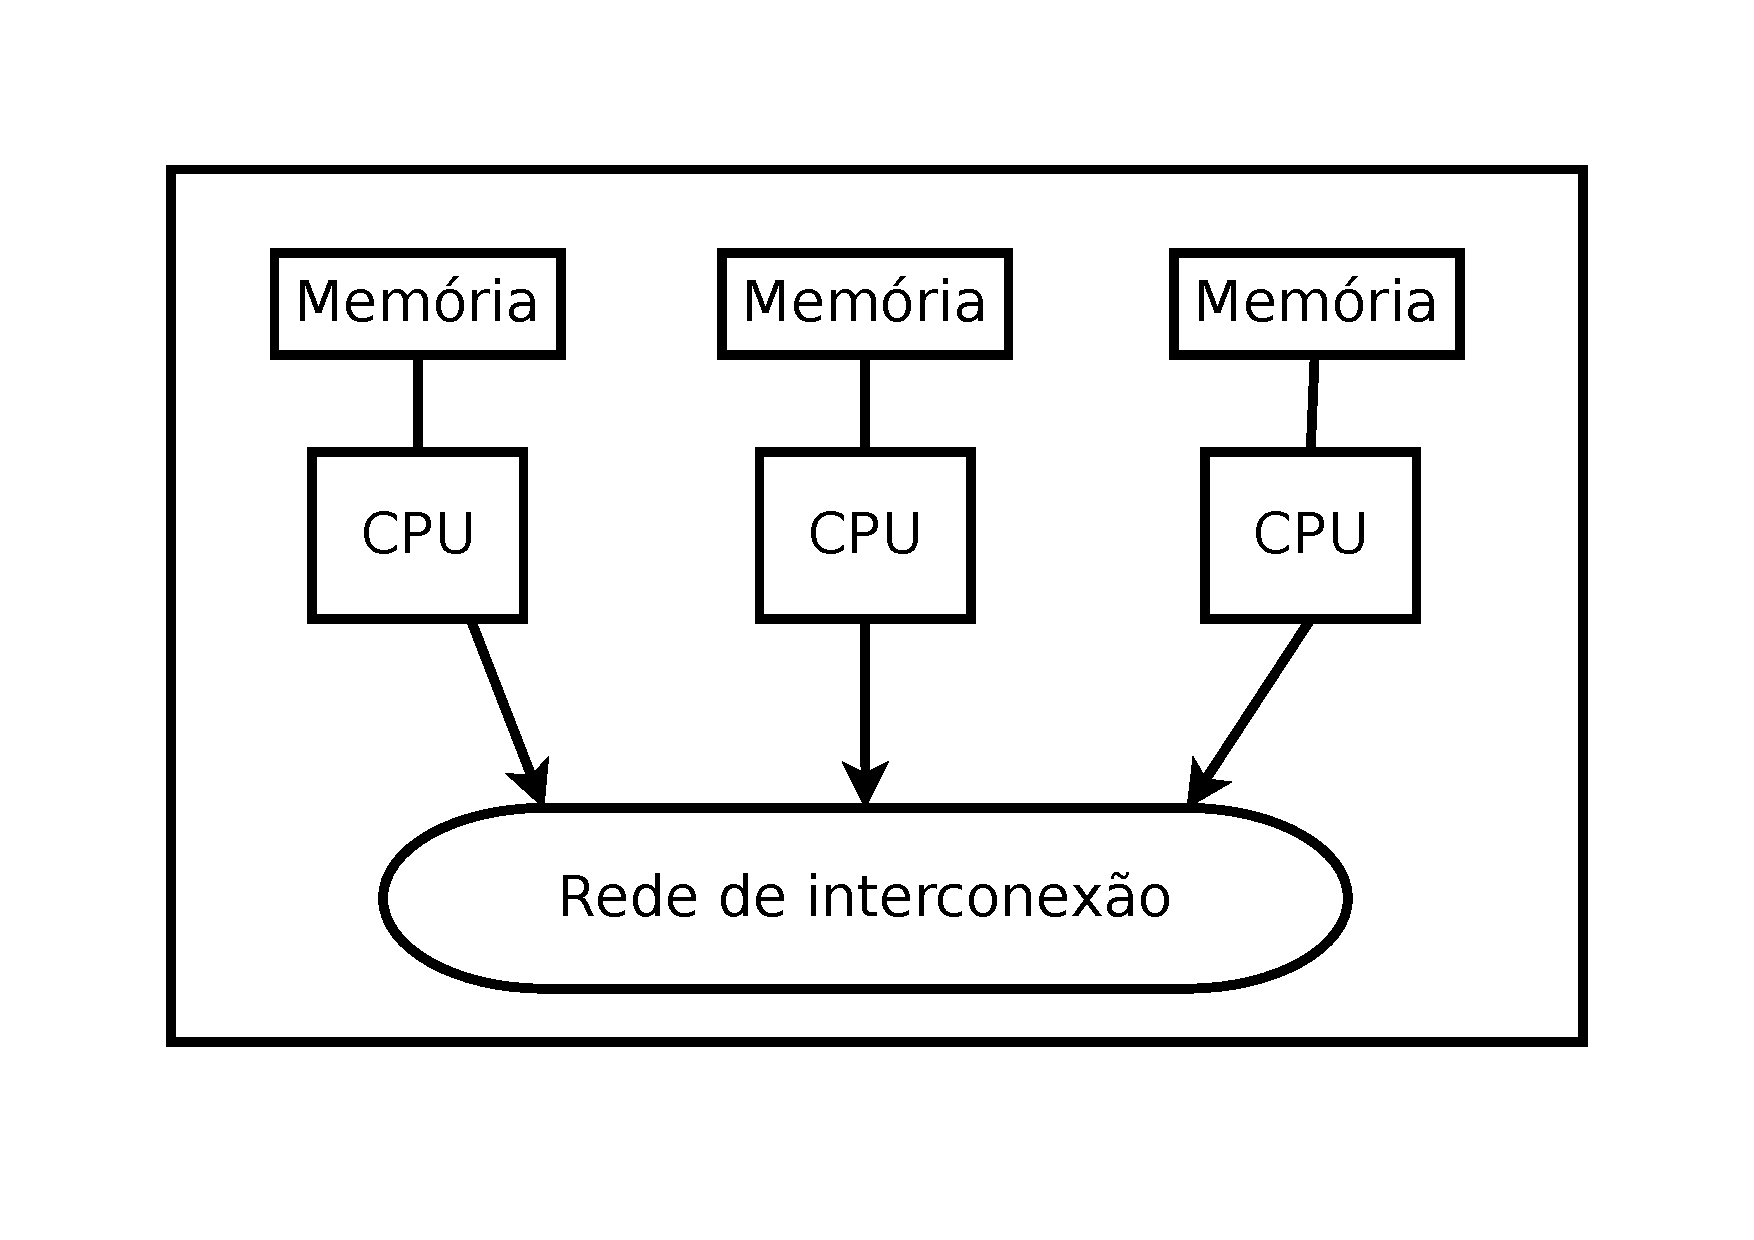
\includegraphics[trim=0cm 1cm 0cm 0cm, width=0.5\textwidth]{figuras/Arquitetura.pdf}
\caption{Modelo de arquitetura distribuída}
\label{fig:ArquiteturaDistribuida}
\end{figure}

\subsection{Computação paralela em \textit{clusters}}
Com o avanço tecnólogico da última década, o volume crescente de dados gerados, coletados e armazenados tornou o processamento dos dados inviável a um único computador.
A necessidade de manipular tais volumes de dados coloca em foco a computação de grandes volumes de dados, que requerem alto desempenho, em detrimento do modelo de processamento massivo em CPU.  Como resultado, torna-se crucial substituir a computação tradicional por computação distribuída eficiente, e é um caminho natural para o processamento de dados em larga escala o uso de \textit{clusters} ~\cite{Lin:2010}.

\textit{Clusters} são conjuntos de máquinas, ligadas em rede, que comunicam-se através do sistema, trabalhando como se fossem uma única máquina de grande porte. 
Dentre algumas características observadas em um \textit{cluster}, é possível destacar: o baixo custo se comparado a supercomputadores; a proximidade geográfica dos nós; altas taxas de transferência nas conexões entre as máquinas e o uso de máquinas em geral homogêneas \cite{Toth:2008}.

Apesar dos computadores em um \textit{cluster} não precisarem processar necessariamente a mesma aplicação, a grande vantagem de tal organização é a habilidade de cada nó processar individualmente uma fração da aplicação, resultando em desempenho que pode ser comparado ao de um supercomputador.
Em geral os computadores de \textit{clusters} são de baixo custo, o que permite que um grande número de máquinas seja interligado, garantindo desempenho e melhor custo-benefício que os supercomputadores, o que apresenta outra vantagem. Além disso, novas máquinas podem ser facilmente incorporadas  ao \textit{cluster}, tornando-o uma solução mais flexível, principalmente por ser formado por máquinas de capacidade de processamento similar.

O bom desempenho das aplicações em \textit{clusters} envolve conceitos relacionados à infraestrutura, principalmente comunicação entre os nós e balanceamento de carga.
Para que o processamento do \textit{cluster} possa ser utilizado de maneira eficiente, é importante que os dados a serem processados sejam transferidos suficientemente rápidos, através de redes de alta velocidade, para evitar que os processadores fiquem ociosos o, subutilizando o poder de processamento do \textit{cluster}.\cite{Rauber:2010}. 


\subsection{Computação paralela em grandes volumes de dados}
O processamento em \textit{clusters} é uma tarefa cujo desempenho é dependente de diversos fatores, como descrito anteriormente. O processamento de grandes volumes de dados também é uma tarefa desafiadora, que tem sido objeto de vários estudos. Os sistemas utilizados para processar grandes volumes de dados devem se basear em alguns princípios para garantir a escalabilidade e o bom desempenho.

A coleta e manutenção dos dados devem ser funções do sistema e não tarefa dos usuários. O sistema deve prover tratamento intrínseco dos dados  e os usuários devem ter facilidade para acessá-los. Mecanismos de confiabilidade, como replicação e  correção de erros devem ser incorporados como parte do sistema de modo a garantir integridade e disponibilidade dos dados.
O uso de modelos de programação paralela de alto nível também deve ser incentivado. O desenvolvedor deve utilizar programação de alto nível que não inclua configurações específicas de uma máquina. O trabalho de distribuir a computação entre as máquinas de forma eficiente deve ficar a cargo do sistema, e não do desenvolvedor.

%Os usuários devem ser capazes de executar programas de forma interativa, com variação dos requisitos de computação e armazenamento. O sistema deve responder rapidamente à consultas e cálculos simples, e não degradar o desempenho geral quando a tarefa for complexa. 
%Para suportar a computação interativa, deve haver oferta de recursos. O custo consequente do aumento dos recursos ofertados pode ser justificado com base no aumento da produtividade dos usuários do sistema.

Além disso, um sistema para computação de grandes volumes de dados deve implementar mecanismos de confiabilidade, no qual os dados originais e intermediários sejam armazenados de forma redundante. Isso permite que no caso de falhas de componente ou dados seja possível refazer a computação. Além disso, a máquina deve identificar e desativar automaticamente componentes que falharam, de modo a não prejudicar o desempenho do sistema e se manter sempre disponível \cite{Bryant:2011}.

Grandes empresas de serviços de Internet - como Google, Yahoo!, Facebook e Amazon - buscam soluções para processamento de dados em grandes conjuntos de máquinas que atendam as características descritas, pois com um software que possa prover tais características é possível alcançar alto grau de escalabilidade e custo-benefício. 

Dentre as principais propostas está o modelo MapReduce e sua implementação Hadoop, que são soluções escaláveis, capazes de processar grandes volumes de dados, com alto nível de abstração para distribuir a aplicação e mecanismos de tolerância a falhas.
A próxima seção apresenta com mais detalhes o modelo e suas características.

\section{MapReduce}
O MapReduce é um modelo de programação paralela criado pela Google para processamento de grandes volumes de dados em \textit{clusters}. Esse modelo propõe simplificar a computação paralela e ser de fácil uso, abstraindo conceitos complexos da paralelização - como tolerância a falhas, distribuição de dados e balanceamento de carga - e utilizando duas funções principais: Map e Reduce. Os princípios do desenvolvimento paralelo não são vistos pelo desenvolvedor, que pode se ocupar em desenvolver a solução proposta \cite{Dean:2008}.

Esse modelo de programação é inspirado em linguagens funcionais, tendo como base as primitivas Map e Reduce.
Os dados de entrada são específicos para cada aplicação e descritos pelo usuário.
A função Map é aplicada aos dados de entrada e produz uma lista intermediária de pares (chave, valor). Todos os valores intermediários associados a uma mesma chave são agrupados e enviados à função Reduce.
A função Reduce então
%aplicada a todos os pares intermediários com a mesma chave. A função
combina esses valores para formar um conjunto menor de resultados.
Tipicamente há apenas zero ou um valores de saída em cada função Reduce. Esses valores são agrupados na forma de pares no formato (chave, valor), que representam a saída da função.

O pseudocódigo a seguir apresenta um exemplo de uso do MapReduce, cujo objetivo é contar a quantidade de ocorrências de cada palavra em um documento. A função Map recebe como valor uma linha do documento, e como chave o número da linha. Para cada palavra encontrada na linha recebida, a função emite a palavra e a contagem de uma ocorrência. A função Reduce, recebe como chave uma palavra, e uma lista dos valores emitidos pela função Map, associados com a palavra em questão. As ocorrências da palavra são agrupadas e a função retorna a palavra e seu total de ocorrências.

\begin{lstlisting}[label=some-code,caption=Pseudocódigo para contagem de palavras no modelo MapReduce]
Function Map (Integer chave, String valor):
	#chave: número da linha no arquivo.
	#valor: texto da linha correspondente.
	listaDePalavras = split (valor)
	for palavra in listaDePalavras:
		emit (palavra, 1)
Function Reduce (String chave, Iterator valores):
	#chave: palavra emitida pela função Map.
	#valores: conjunto de valores emitidos para a chave.
	total = 0
	for v in valores:
		total = total + 1
	emit (palavra, total)
\end{lstlisting}

A Figura \ref{fig:MapReduceexemplo} ilustra o fluxo de execução para este exemplo. A entrada é um arquivo contendo as linhas "hadoop conta", "conta palavras" e "exemplo hadoop".

\begin{figure}[htb]
\centering
%trim left, bottom, right and top
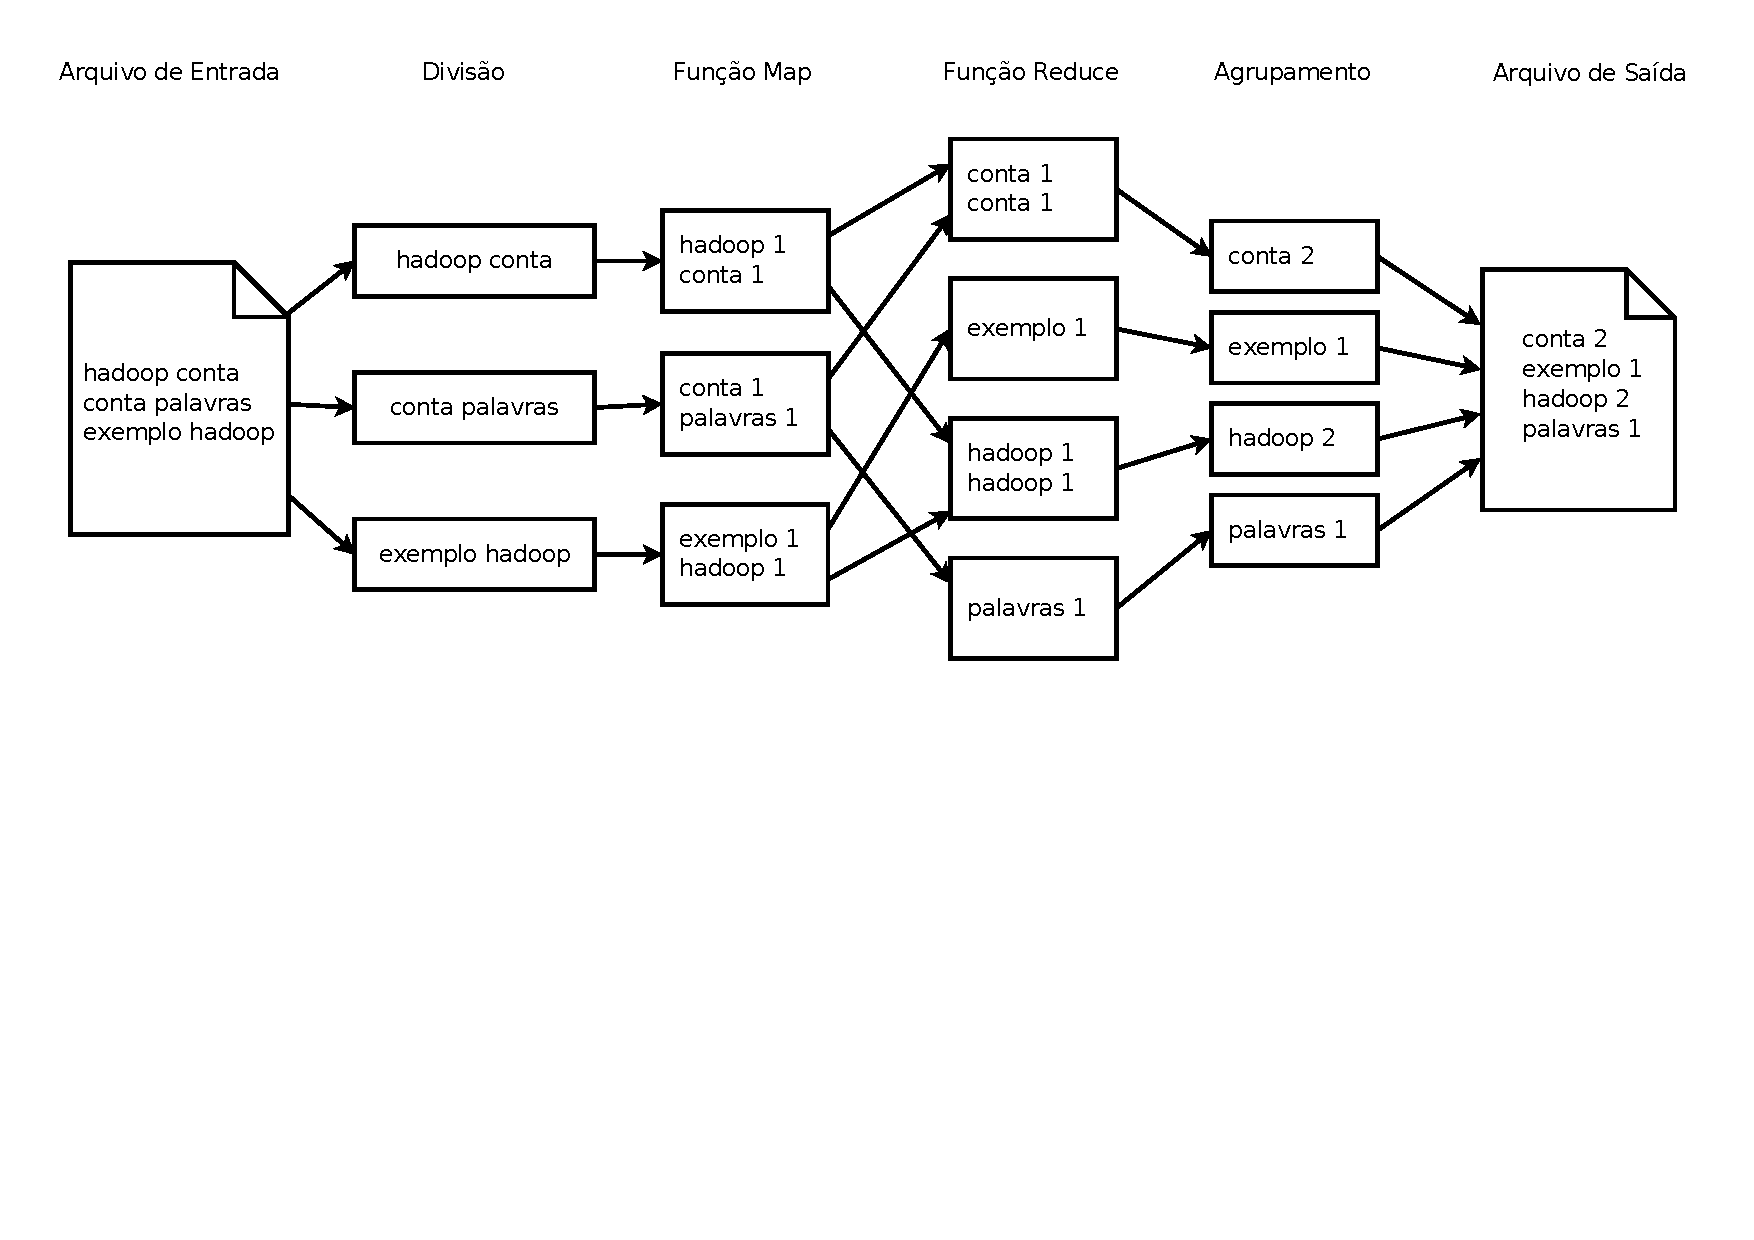
\includegraphics[trim=0cm 9cm 0cm 1cm, width=\textwidth]{figuras/MapReduceExemplo.pdf}
\caption{Exemplo da contagem de palavras com o MapReduce}
\label{fig:MapReduceexemplo}
\end{figure}

\subsection{Arquitetura do MapReduce}
O MapReduce é constituído de uma arquitetura com dois tipos principais de nós: \textit{Master} e \textit{Worker}. O nó mestre tem como função atender requisições de execução dos usuários, gerenciá-las, criar tarefas e distribuí-las entre os nós trabalhadores, que executam as tarefas com base nas funções Map e Reduce definidas pelo usuário.
%Como é possível perceber, trata-se de uma típica arquitetura mestre-escravo (do inglês master-slave) (DUBREUIL; GAGNÉ; PARIZEAU, 2006).
A arquitetura também inclui um sistema de arquivos distribuídos, onde ficam armazenados os dados de entrada e intermediários.
%Para evitar a transferência excessiva de dados, os \textit{workers} do MapReduce são também nós do sistema de arquivos.


% }

\subsection{Visão geral do fluxo de execução}


As chamadas da função Map são distribuídas automaticamente entre as diversas máquinas através do particionamento dos dados de entrada em \textit{M} conjuntos. Cada conjunto pode ser processado em paralelo por diferentes máquinas. As chamadas da função Reduce são distribuídas pelo particionamento do conjunto intermediário de pares em \textit{R} partes. O número de partições \textit{R} pode ser definido pelo usuário.

A Figura \ref{fig:MapReduceoverview} ilustra o fluxo de uma execução do modelo MapReduce \cite{Dean:2008}. A sequência de ações descrita a seguir explica o que ocorre em cada um dos passos. A numeração dos itens a seguir corresponde à numeração da figura.

 \begin{figure}[!htb]
 \centering
%trim left, bottom, right and top
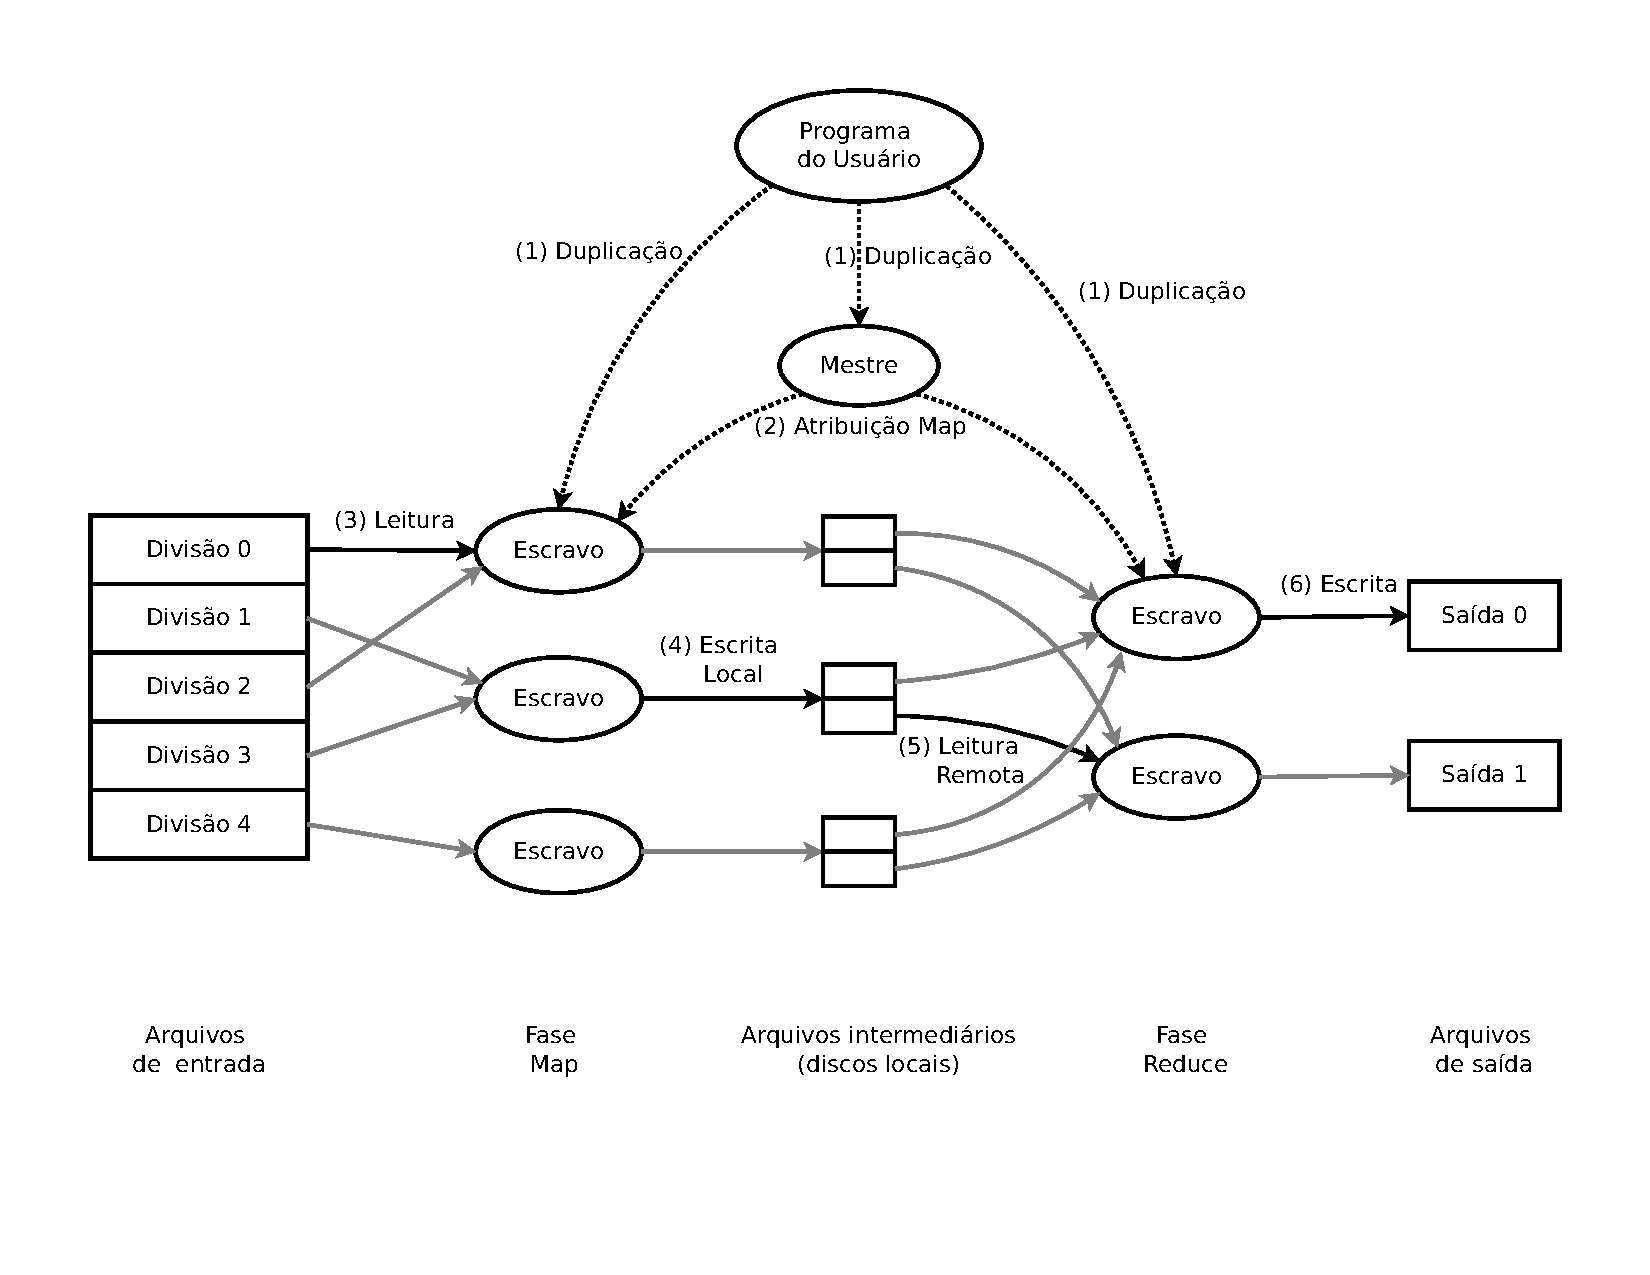
\includegraphics[trim=0cm 2cm 0cm 1cm, width=\textwidth]{figuras/MapReduceOverflow.pdf}
\caption{Visão geral do funcionamento do modelo MapReduce.}
\label{fig:MapReduceoverview}
\end{figure}

\begin{enumerate}
\item A biblioteca MapReduce, no programa do usuário, divide os arquivos de entrada em M pedaços. Em seguida, iniciam-se muitas cópias do programa para o conjunto de máquinas;

\item Uma das cópias do programa é especial: o mestre (\textit{Master}). Os demais são trabalhadores (\textit{Workers}) cujo trabalho é atribuído pelo mestre. Existem M tarefas Map e R tarefas Reduce a serem atribuídas. O mestre atribui aos trabalhadores ociosos uma tarefa Map ou uma tarefa Reduce;

\item Um trabalhador que recebe uma tarefa Map lê o conteúdo do fragmento de entrada correspondente. Ele cria pares (chave, valor) a partir dos dados de entrada e encaminha cada par para a função Map definida pelo usuário. Os pares (chave, valor) intermediários, produzidos pela função Map, são colocados no \textit{buffer} de memória;

\item Periodicamente, os pares colocados no \textit{buffer} são gravados no disco local, divididos em R regiões  pela função de particionamento. As localizações desses pares bufferizados, no disco local, são passadas de volta para o mestre que é responsável pelo encaminhamento desses locais aos trabalhadores Reduce;

\item Quando um trabalhador Reduce é notificado pelo mestre sobre essas localizações, ele usa chamadas de procedimento remoto para ler os dados dos discos locais dos trabalhadores Map. Quando um trabalhador Reduce tiver lido todos os dados intermediários da sua partição, ele a ordena pelas chaves intermediárias, de forma que todas as ocorrências da mesma chave estejam agrupadas. Se a quantidade de dados intermediários é muito grande para caber na memória, um tipo de ordenação externa é usado;

\item O trabalhador Reduce itera sobre os dados intermediários ordenados e, para cada chave encontrada, repassa a chave e o conjunto correspondente de valores intermediários para função Reduce do usuário. A saída da função Reduce é anexada a um arquivo de saída final para essa partição Reduce;

             	        	
\end{enumerate}

Após todas as tarefas Map e Reduce concluídas, o mestre acorda o programa do usuário, retornando, neste ponto, a chamada MapReduce para o código do usuário.

\section{Hadoop}

O Hadoop é uma das  implementações mais conhecidas modelo MapReduce. Ele provê o gerenciamento de computação distribuída, de maneira escalável e confiável. É uma implementação código aberto em Java  desenvolvida por Doug Cutting em 2005 e mantida pela Apache Software Foundation \cite{White:2009, Hadoop:2010}.

Um dos principais benefícios do Hadoop é permitir o processamento em conjunto de centenas de máquinas de maneira transparente, o que significa que o usuário não deve se preocupar com mecanismos de tolerância a falhas, que é provido pelo sistema. %\cite{Dean:2008}. 
Facebook, Yahoo! e eBay utilizam o ambiente Hadoop em seus \textit{clusters}, para processar diariamente terabytes de dados e logs de eventos para detecção de \textit{spam}, \textit{business intelligence} e diferentes tipos de otimização \cite{Cherkasova:2011}.

O mecanismo de tolerância a falhas implementado pelo sistema, permite que o trabalho do usuário possa ser concluído mesmo que ocorra alguma falha de disco, de processo ou de nó. Periodicamente, o nó mestre envia mensagens aos demais nós para verificar seus estados. Se nenhuma resposta é recebida, o mestre identifica que houve falha neste nó e o substitui. 
As tarefas que não foram executadas são reescalonadas para os demais nós. O mecanismo de replicação garante que sempre haja um número determinado de cópias dos dados, e caso um dos nós de armazenamento seja perdido, os demais se encarregam de realizar uma nova replicação \cite{White:2009}.
 % O sistema é capaz de verificar e substituir nós quando ocorre alguma falha. 


\subsection{Sistema de Arquivos do Hadoop}


O \textit{ Hadoop Distributed File System} (HDFS) é um sistema de arquivos distribuído desenvolvido para armazenar grandes conjuntos de dados e ser altamente tolerante a falhas \cite{White:2009}.
A plataforma Hadoop fornece o HDSF como sistema de arquivos padrão, mas é compatível com diversos sistemas de arquivos distintos, como Amazon S3 (Native e Block-based), CloudStore, HAR, Local (destinado a unidades de armazenamento conectadas localmente) e sistemas mantidos por servidores FTP e HTTP.

A arquitetura do HDFS também é do tipo mestre-escravos. 
O nó mestre consiste em um \textit{JobTracker}  para as tarefas MapReduce e um \textit{NameNode}  responsável por manter e controlar todos os metadados do sistema de arquivos e gerenciar a localização dos dados. O nó mestre também é responsável por outras atividades, como por exemplo, balanceamento de carga, \textit{garbage collection} e atendimento a requisições dos clientes.
Os nós escravos são formados por um \textit{TaskTracker}  para as tarefas MapReduce e por um \textit{DataNode} responsável por armazenar e transmitir os dados aos usuários que os requisitarem.

A Figura \ref{fig:hdfs} ilustra a arquitetura do sistema de arquivos distribuídos.
O \textit{NameNode} gerencia e manipula todas as informações dos arquivos, tal como a localização e o acesso. Os \textit{DataNodes} se encarregam da leitura e escrita das informações nos sistemas de arquivo cliente. Os \textit{JobTracker} e \textit{TaskTracker} são responsáveis por executar as tarefas MapReduce.
\begin{figure}[htb]
\centering
%trim left, bottom, right and top
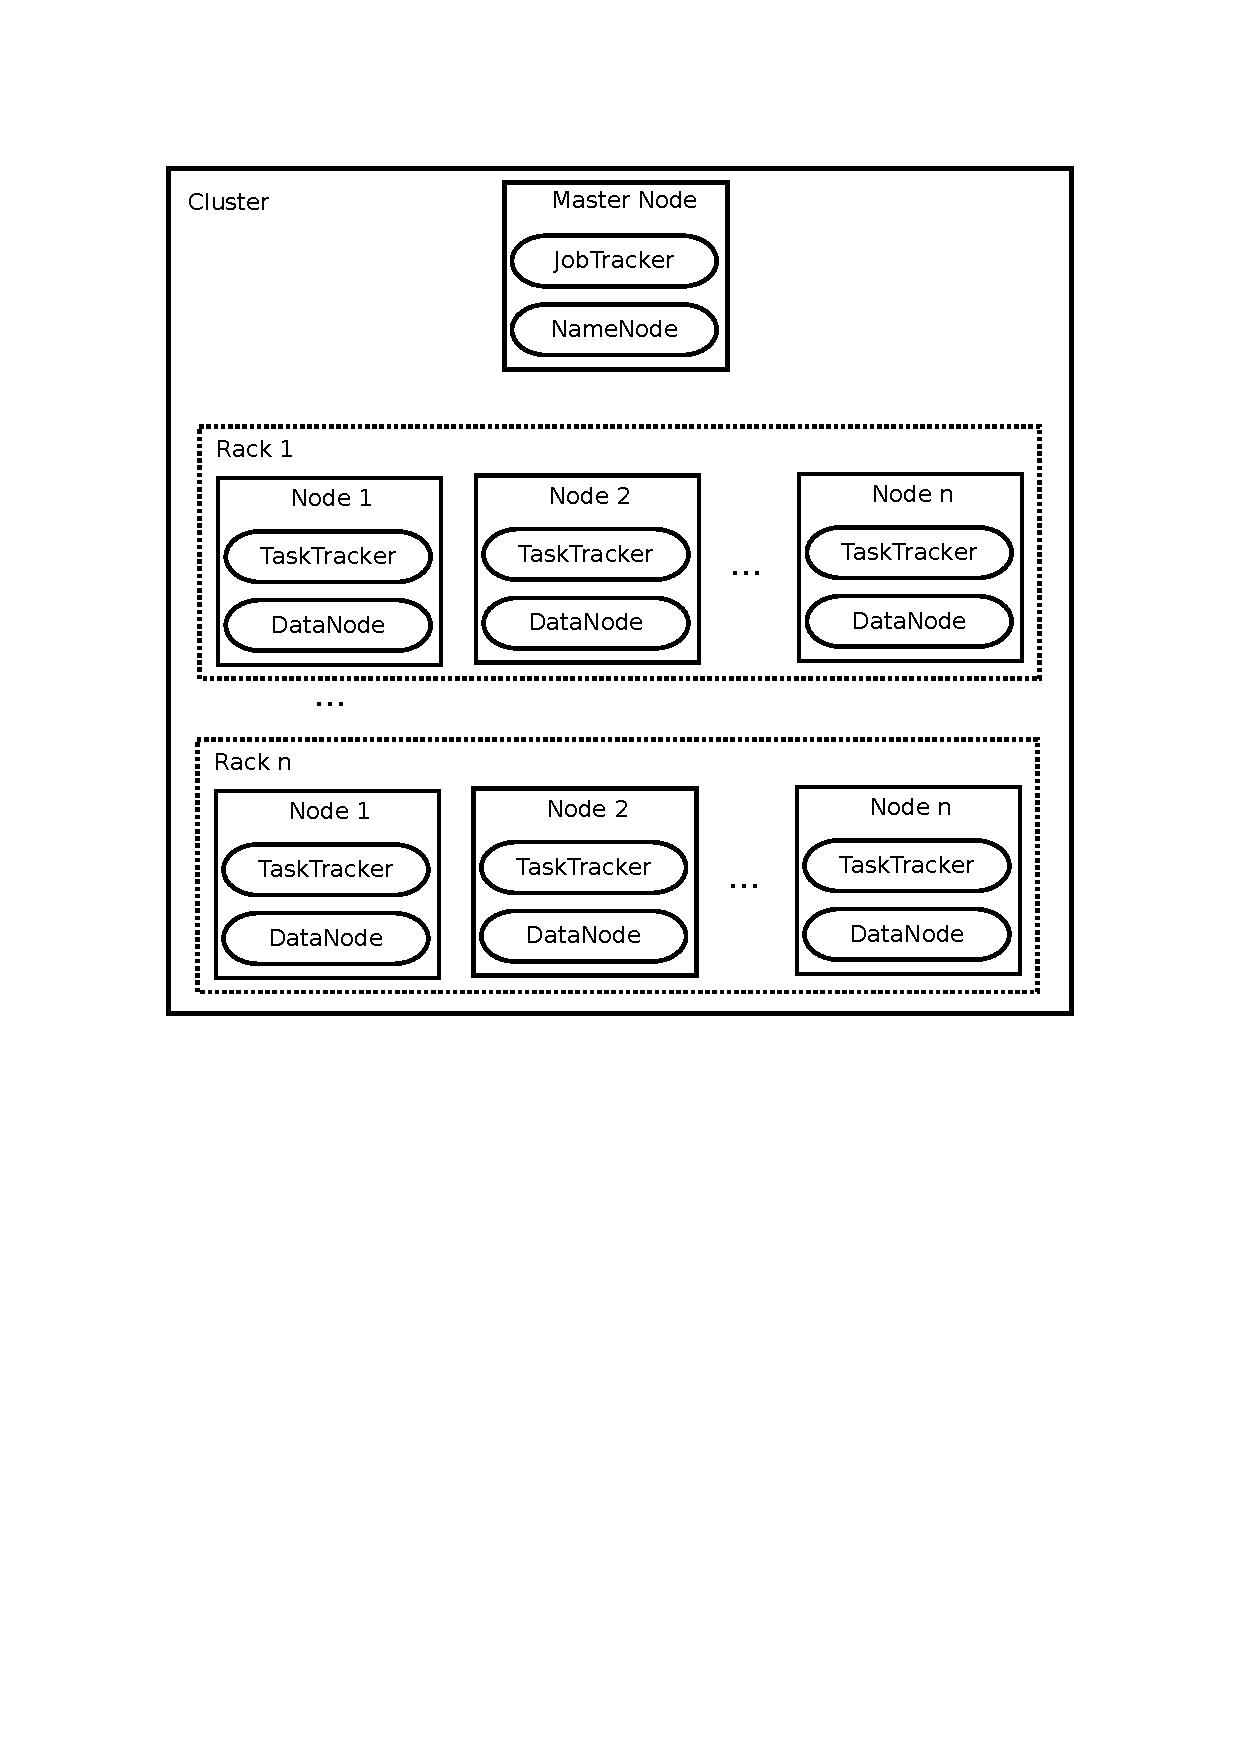
\includegraphics[trim=2cm 12cm 2cm 2cm, width=0.6\textwidth]{figuras/HadoopCluster.pdf}
\caption{Visão abstrata do cluster.}
\label{fig:hdfs}
\end{figure}

O HDFS incorpora funcionalidades que têm grande impacto no desempenho geral do sistema.
Uma delas é conhecida como \textit{rack awareness}. Com esse recurso, o sistema de arquivos é capaz de identificar os nós escravos que pertencem a um mesmo \textit{rack}, e distribuir as réplicas de maneira mais inteligente, aumentando o desempenho e a confiabilidade do sistema.
Outra funcionalidade é a distribuição das tarefas considerando localização dos dados nos nós. O sistema de arquivos procura manter um balanceamento na ocupação das unidades de armazenamento, e o \textit{framework} busca atribuir tarefas a um escravo que possua, em sua unidade de armazenamento local, os dados que devem ser processados.
Assim, quando executa-se grandes operações MapReduce com um número significativo de nós, a maioria dos dados são lidos localmente e o consumo de banda é mínimo.		% Fundamentação teórica
	%
% Documento: Trabalhos Relacionados
%
\chapter{Ordenação de Dados}
\label{cap:ordenacao}


A ordenação é o processo de organizar elementos de uma sequência em determinada ordem, considerada um dos problemas fundamentais da computação devido à sua importância teórica e prática \cite{Knuth:1998, Cormen:2009}. 
A ordenação é utilizada por um grande número de aplicações computacionais, como compiladores e sistemas operacionais, que usam extensivamente a ordenação para lidar com tabelas e listas. 
A construção de estruturas essenciais em computação gráfica e sistemas de informação geográfica são fundamentalmente operações de ordenação, que também participam de aplicações como a compressão de dados. A ordenação ainda é utilizada para determinar a duplicidade de elementos, encontrar o maior valor, realizar busca contínua e por operações SQL, que internamente a utilizam na criação de índices e buscas binárias. Dessa forma, diversos sistemas e bancos de dados se beneficiariam de uma rotina eficiente de ordenação \cite{Lauterbach:2009,Satish:2009,Dean:2008}.


De forma geral, a ordenação pode ser dividida em dois grupos: ordenação interna e externa. 
A ordenação em memória interna é caracterizada pelo armazenamento de todos os registros na memória principal, onde seus acessos são feitos diretamente pelo processador. Essa ordenação é possível apenas quando a quantidade de dados é pequena o suficiente para ser armazenada em memória. 

Quando é preciso ordenar uma base de dados muito grande, que não cabe na memória principal, um outro modelo faz-se necessário, a ordenação externa.
Apesar do problema nos dois casos ser o mesmo - rearranjar os registros de um arquivo em ordem ascendente ou descendente - não é possível usar as mesmas estratégias da ordenação interna, pois o acesso aos dados precisa ser feito em memória secundária, basicamente discos, cujo tempo de acesso é várias ordens de grandeza superior ao da memória principal.  %[Ziviani 2007, Knuth 1973].

Na ordenação externa, os itens que não estão na memória principal devem ser buscados em memória secundária e trazidos para a memória principal, para assim serem comparados. Esse processo se repete numerosas vezes, o que o torna lento, uma vez que os processadores ficam grande parte do tempo ociosos à espera da chegada dos dados à memória principal para processá-los. Por esse motivo, a grande ênfase de um método de ordenação externa deve ser a minimização do número de vezes que cada item é transferido entre a memória interna e a memória externa. Além disso, cada transferência deve ser realizada de forma tão eficiente quanto as características dos equipamentos disponíveis permitam \cite{Ziviani:2007}.


\section{Ordenação Paralela}


Diversas aplicações possuem uma fase de processamento intenso, na qual é preciso ordenar uma lista de elementos. Mesmo algoritmos de ordenação sequenciais ótimos, como o \textit{Quicksort} e o \textit{HeapSort}, apresentam custo mínimo ${\cal O}(n/log \quad n)$ para ordenar uma sequência de $n$ chaves \cite{Cormen:2009}. 
Isso significa que, com o crescimento do número de elementos a ser ordenado, o tempo para realizar a ordenação aumenta de maneira não linear, o que pode ser um entrave ao processamento. 
A fim de resolver tal problema, com o surgimento do processamento paralelo, foram apresentadas versões paralelas dos algoritmos de ordenação sequenciais, com o intuito de diminuir consideravelmente o tempo de execução. A importância da ordenação têm originado estudos buscando desenvolver algoritmos de ordenação eficientes para uma grande variedade de arquiteturas paralelas \cite{Akl:1990}.

\textbf{A ordenação paralela} é o processo  de ordenação feito em múltiplas unidades de processamento, que trabalham em conjunto para ordenar uma sequência de entrada. O conjunto inicial é dividido em subconjuntos disjuntos, que são associados a uma única unidade de processamento. A sequência final ordenada é obtida a partir da composição dos subconjuntos ordenados. É um ponto fundamental do algoritmo de ordenação paralela que a distribuição dos dados a serem ordenados, em cada processo individual, seja feita de tal forma que todas as unidades de processamento estejam trabalhando e que o custo de redistribuição de chaves entre os processadores seja minimizado. 

\textbf{A ordenação paralela} é uma aplicação estudada intensivamente desde o início da computação paralela, com primeiro método \textit{Bitonic Sorting Network} proposto por Batcher \cite{Batcher:1968}. 
Estudos teóricos foram realizados inicialmente, mas testes empíricos se tornaram possíveis na década de 80 com a disponibilidade de arquiteturas vetoriais, de multiprocessadores e multicomputadores e diversas versões paralelas dos algoritmos \textit{Quicksort}, \textit{RadixSort} e \textit{MergeSort} foram propostas.


O \textit{Quicksort} Paralelo foi um dos algoritmos mais estudados \cite{Deminet:1982, Quinn:1994, Sanders:1997}, mas inicialmente a divisão dos dados limitava o aumento da velocidade, independente do número de processadores utilizados. Recentemente novas implementações foram propostas, utilizando as tecnologias  de \textit{hyperthreading} disponíveis em processadores atuais para desenvolver um esquema de balanço de carga, que têm se mostrado eficiente na divisão dos dados \cite{Parikh:2008}.
Para o \textit{MergeSort} foi proposta uma versão chamada \textit{Simple Randomized Mergesort} \cite{Barve:1996, Barve:2002}, que foi o primeiro algoritmo de ordenação em disco a obter um número médio ótimo de movimentações de dados. 
 A implementação \textit{Quickmerge} proposta por Quinn combinava os algoritmos \textit{Quicksort} e \textit{MergeSort}, reduzindo significativamente a quantidade de dados movimentada \cite{Quinn:1988}. Também foram estudados algoritmos de ordenação paralela que se baseiam em uma amostra para realizar a divisão do conjunto de dados. Podem ser citados o \textit{FlashSort} \cite{Reif:1987}, o \textit{Samplesort} \cite{Huang:1983} e suas variações como o \textit{Super-Scalar Samplesort }\cite{Sanders:2004} e o \textit{Parallel Sorting by Regular Sampling} \cite{Shi:1992}.

Além disso, as propostas atuais de ordenação em grandes conjuntos de máquinas incluem os algoritmos implementados em Hadoop \textit{Sort} e \textit{TeraSort}, descritos na seção \ref{sec:benchmarks}, capazes de ordenar petabytes de informação em centenas ou milhares de nodos. 



Com tamanha variedade de algoritmos e arquiteturas, diversas soluções podem ser consideradas ao implementar um algoritmo de ordenação em ambiente paralelo. Cada uma delas atende um cenário, tipo de entrada, plataforma ou arquitetura particulares. Dessa forma, ao desenvolver algoritmos de ordenação paralela, é importante ter em mente certas condições que interferem no desempenho final do algoritmo, relacionadas tanto ao ambiente de implementação, quanto ao conjunto de dados que deve ser ordenado. As principais questões a serem analisadas são \cite{Kale:2010}:

\begin{itemize}
\item \textbf{Habilidade de explorar distribuições iniciais parcialmente ordenadas:}
Alguns algoritmos podem se beneficiar de cenários nos quais a sequência de entrada dos dados é a mesma, ou pouco alterada. Nesse caso, é possível obter melhor desempenho ao realizar menos trabalho e movimentação de dados.
Se a alteração na posição dos elementos na sequência é pequena o suficiente, grande parte dos processadores mantém seus dados iniciais e precisam se comunicar apenas com os processadores vizinhos.

\item \textbf{Movimentação dos dados:}
A movimentação de dados entre processadores deve ser mínima durante a execução do algoritmo. Em um sistema de memória distribuída, a quantidade de dados a ser movimentada é um ponto crítico, pois o custo de troca de dados pode dominar o custo de execução total e limitar a escalabilidade.

\item \textbf{Balanceamento de carga:}
O algoritmo de ordenação paralela deve assegurar o balanceamento de carga ao distribuir os dados entre os processadores. Cada processador deve receber uma parcela equilibrada dos dados para ordenar, uma vez que o tempo de execução da aplicação é tipicamente limitada pela execução do processador mais sobrecarregado.

\item \textbf{Latência de comunicação:}
A latência de comunicação é definida como o tempo médio necessário para enviar uma mensagem de um processador a outro.
Em grandes sistemas distribuídos, reduzir o tempo de latência se torna muito importante.

\item \textbf{Sobreposição de comunicação e computação:}
Em qualquer aplicação paralela, existem tarefas com focos em computação e comunicação. A sobreposição de tais tarefas permite que sejam feitas tarefas de processamento e ao mesmo tempo operações de entrada e saída de dados, evitando que os recursos fiquem ociosos durante o intervalo de tempo necessário para a transmissão da carga de trabalho.

\end{itemize}


Além das condições relacionadas à implementação do algoritmo em ambiente paralelo, existem outras condições necessárias, relacionadas principalmente ao conjunto de elementos a ser ordenado. Considerando um conjunto de $n$ chaves e  $p$ processadores,  durante a execução de qualquer algoritmo de ordenação paralela é preciso que o conjunto de chaves seja particionado em $p$ subconjuntos mutualmente exclusivos, sem nenhuma chave duplicada. É necessário ainda que todas as chaves da sequência inicial sejam mantidas, ou seja, que não se perca nenhuma chave durante a distribuição entre os processadores.

Após o conjunto estar ordenado, é preciso verificar se todas as chaves da sequência inicial foram preservadas, se todas as chaves de cada processador estão ordenadas em ordem crescente, se a maior chave no processador $p_{i}$ é inferior ou igual à menor chave no processador $p_{i+1}$ e se a saída resultante é uma sequência de chaves totalmente ordenada.

\subsection{Fluxo geral de execução da ordenação paralela}

Na execução de um algoritmo de ordenação paralela podem ser identificadas algumas tarefas principais, que todos os algoritmos precisam executar em algum momento, normalmente realizadas de forma sequencial  \cite{Kale:2010}. 
A primeira tarefa é a ordenação local, na qual as chaves em cada processador são ordenadas inicialmente  ou ordenadas em grupos.
Existe também uma fase de agrupamento, pois muitas vezes é necessário colocar as chaves em grupos, a fim de enviá-las a outros processadores ou calcular histogramas. Por fim, é preciso realizar a intercalação das chaves ordenadas em subsequências em uma sequência completa.

Os algoritmos de ordenação paralela executam tarefas similares que podem ser definidas, genericamente, como se segue: 
\begin{num_enum}
\item Realizar processamento local;
\item Coletar informações relevantes de distribuição de todos os processadores;
\item Em um único processador, inferir uma divisão de chaves a partir das informações coletadas;
\item Transmitir aos outros processadores a divisão dos elementos;
\item Realizar processamento local;
\item Mover os dados de acordo com os elementos de divisão;
\item Realizar processamento local;
\item Se a divisão de chaves foi incompleta, retornar ao passo 1;
\end{num_enum}


De acordo com essa generalização  é possível identificar pontos que se relacionam diretamente com as condições que limitam o desempenho dos algoritmos de ordenação paralela e fornecem ideias para a análise de eficiência da comunicação dos algoritmos.
Primeiro, há duas tarefas principais de comunicação: descobrir um vetor de divisão global e enviar os dados para os processadores adequados. 
Em segundo lugar, a maioria dos algoritmos têm múltiplos estágios de computação local e pode ser muito vantajoso sobrepor este processamento local e a comunicação. 
%Finalmente, se é possível realizar sobreposição entre o processamento local e a determinação do vetor de divisão, um processador pode ser reservado para o trabalho de divisão, encurtando o caminho crítico. 
A fração de  processamento local que pode ser sobreposta à comunicação necessária em um algoritmo  é um bom indicativo para comparação da escalabilidade dos algoritmos de ordenação paralela.
%ao custo para determinar a divisão e mover os dados


\section{Algoritmos de Ordenação Paralela}

Essa seção apresenta os algoritmos de ordenação paralela objetos desse trabalho: o algoritmo Ordenação por Amostragem  (\textit{Samplesort}) e o algoritmo \textit{Quicksort} Paralelo, bem como as aplicações de ordenação em Hadoop \textit{Terasort} e \textit{Sort}.  

%%% EXEMPLO
%A Figura 4.3 mostra três etapas de particionamento de um vetor de dez chaves inteiras. A primeira linha mostra os dados originais; a segunda mostra os dados após o vetor ter sido particionado; e a terceira mostra como cada uma das duas partições, a partir da segunda linha, seria particionada. As caixas encapsulam as partes do vetor que precisam ser ordenadas.

\subsection{Ordenação no ambiente Hadoop}
\label{sec:benchmarks}
A ordenação de dados é uma das cargas de trabalho mais consideradas pelos \textit{benchmarks} em geral, que buscam, a partir de uma entrada desordenada, obter uma saída ordenada e avaliar o desempenho do algoritmo que realizou a ordenação.

% O \textit{framework} Hadoop disponibiliza diversos programas que podem ser facilmente executados, dentre os quais se destacam o \textit{Sort} e o \textit{TeraSort}.
O \textit{Sort} é um \textit{benckmark} criado por Jim Gray em 1998, e hoje é um dos mais conhecidos na ordenação de dados \cite{Gray:1998}. 
Consiste em um conjunto de seis \textit{benchmarks}, cada um com as suas regras, que medem os tempos para ordenar diferentes números de registros e se diferem principalmente nas métricas de avaliação. 
As principais categorias dos \textit{benchmarks Sort} são a \textit{MinuteSort} e a \textit{GraySort}. A categoria \textit{MinuteSort} deve ordenar a maior quantidade dos dados em um minuto e a \textit{GraySort} deve ordenar mais que 100 terabytes em pelo menos uma hora \cite{White:2009}. Ainda existem as categorias \textit{PennySort}, \textit{JouleSort}, e os descontinuados  \textit{DatamationSort} e \textit{TeraByte Sort}. 
Em cada categoria de ordenação, existem duas classificações, de acordo com o tipo de registro a ser ordenado: \textit{Daytona} e \textit{Indy}. Os participantes da categoria \textit{Daytona} são códigos de ordenação de propósito geral, e os participantes da \textit{Indy} devem ordenar apenas registros de 100 bytes, sendo os primeiros 10 bytes reservados para a chave e o restante compõe o valor do elemento a ser ordenado.


No Hadoop, o \textit{Sort} é uma aplicação MapReduce, composta de três etapas: gerar dados aleatórios, realizar a ordenação e validar os resultados.
A geração de dados aleatórios é feita com o programa \textit{RandomWriter}. Ele executa dez tarefas MapReduce por nó, e cada função Map gera aproximadamente 1GB,  totalizando 10GB de dados binários aleatórios. 
É possível determinar o número de dados e as configurações para os tamanhos das chaves e valores a serem gerados alterando algumas configurações do \textit{RandomWriter}.
No segundo passo é realizada uma ordenação parcial dos dados de entrada e  o resultado é escrito em um diretório de saída. 
O passo final é validar os resultados obtidos pela ordenação dos dados realizada pelo \textit{Sort}, através do programa \textit{SortValidator}, que realiza uma série de verificações nos dados ordenados e nos não ordenados para confirmar se a ordenação foi realizada corretamente. 

Esse programa é muito útil para verificar o desempenho do sistema como um todo, uma vez que todo o conjunto de dados é transferido através da aplicação.

%O Sort é um dos mais conhecidos 
%Os benchmarks relacionados ao Sort possuem uma aplicação MapReduce, que realiza uma ordenação parcial dos dados de entrada, e são constituídos de três passos:
%1. Geração de dados: gera dados aleatórios a serem ordenados;
%2. Ordenação dos dados: ordena os dados gerados pelo passo 1;
%3. Validação de dados: vno passo 2.


O \textit{TeraSort} é outra aplicação de destaque para ordenação de dados com Hadoop, criada por Owen O' Malley \cite{OMalley:2009}, com o intuito de participar da competição \textit{Sort} \cite{Gray:1998}. Em 2009, o \textit{TeraSort} foi o campeão dessa competição em duas categorias: \textit{MinuteSort} ao ordenar 500 GB em 59 segundos, utilizando um \textit{cluster} com 1.406 nodos; e \textit{GraySort} ordenando 100 TB em 173 minutos em um \textit{cluster} com 3.452 nodos. A escalabilidade da solução foi provada pela ordenação de 1 PB em 975 minutos (equivalente a 16,25 horas) em 3.658 nodos.
O \textit{TeraSort} consiste de três algoritmos, que são responsáveis pela geração dos dados, ordenação e validação. 

\textit{Teragen} é o programa padrão para geração dados para a ordenação com \textit{Terasort}.
Nele o número de registros gerados é um parâmetro definido pelo usuário, assim como o número de tarefas Map a serem realizadas. O programa divide o número desejado de registros pelo número de tarefas Map, e atribui a cada tarefa Map um intervalo de chaves para a geração de um arquivo. Cada tarefa Map corresponde a um arquivo de saída, assim os dados gerados são divididos em diversos arquivos. Deste modo, se existem duas tarefas Map, são escritos dois arquivos, cada um contendo metade das chaves geradas. 
Os registros gerados têm um formato específico: uma chave, um id e um valor. As  chaves são caracteres aleatórios do conjunto \mbox{ `` '' .. ``$\sim$''}. O id é um valor inteiro que representa a linha, e o valor consiste de 70 caracteres de `A' a `Z'. 

\textit{TeraSort} é uma espécie MapReduce padrão, mas apresenta um particionador personalizado que usa uma lista ordenada de $ N-1 $ chaves amostradas que definem a faixa de chaves para cada função Reduce. 
Em particular, todas as chaves tal que $amostra [i-1] \le chave < amostra[i] $ são enviadas para a função \textit{i}. 
Isto garante todas as chaves da saída $i$ sejam menores que as da saída $i + 1$ .
Há também um formato de entrada e saída, \textit{TeraOutputFormat}, que é utilizado	 por todas as três aplicações  para ler e gravar os arquivos de texto no mesmo formato. 

\textit{TeraValidate} garante que a saída está totalmente ordenada. A aplicação cria uma função Map para cada arquivo no diretório de saída, que se certifica que cada chave é  menor ou igual à anterior. O Map também gera registros com a primeira e última chave de cada arquivo. Em seguida, a função Reduce lê tais registros e garante que a primeira chave de um arquivo é maior do que a última chave do arquivo anterior. Caso alguma chave seja encontrada fora de ordem, ela é escrita em um  arquivo de saída do Reduce, caso nenhuma chave esteja fora de ordem, não há saídas na função Reduce.

\subsection{Outros}
\label{sec:alg-outros}

O algoritmo \textit{Samplesort} ou Ordenação por Amostragem é um método de ordenação baseado na divisão do arquivo de entrada em subconjuntos, de forma que as chaves de um subconjunto $i$ sejam menores que as chaves do subconjunto $i+1$. Após a divisão, cada subconjunto é enviado a um processador, que ordena os dados localmente. Ao final, todos os subconjuntos são concatenados e formam um arquivo globalmente ordenado.

Nesse algoritmo, o ponto chave é dividir as partições de maneira balanceada, para que cada processador receba aproximadamente a mesma carga de dados. Para isso, é preciso determinar o número de elementos que devem ser destinados a uma certa partição, o que é feito através da amostragem das chaves do arquivo original. Essa estratégia baseia-se na análise de um subconjunto de dados  denominado amostra, ao invés de todo o conjunto, para estimar a distribuição de chaves e construir partições balanceadas.


%O algoritmo Quicksort é um método de ordenação muito rápido e eficiente, inventado por  e publicado em 1962, após uma série de refinamentos [Shustek 2009]. Ele aplica a abordagem 􏰂dividir para conquistar􏰃

O \textit{Quicksort} foi criado por Hoare em 1960 e é considerado o algoritmo de ordenação sequencial mais rápido em grande parte dos casos \cite{Cormen:2009}. É um algoritmo recursivo, que usa a estratégia Dividir para Conquistar para ordenar as chaves.
Na implementação sequencial, a estratégia é o particionamento recursivo da sequência de entrada utilizando um elemento como pivô.  
Após a escolha do elemento pivô, a lista é dividida em duas sublistas, uma contendo elementos iguais e menores que o pivô,  e outra contendo elementos maiores.
Em cada sublista é escolhido um novo pivô e o processo se repete, até que cada lista contenha apenas um elemento.  Ao final obtém-se um conjunto com elementos ordenados. 

Em geral, a complexidade da versão sequencial do algoritmo \textit{Quicksort} é ${\cal O}(n \times log \quad n)$, mas em uma situação em que a entrada de dados seja um  conjunto ordenado ou quase ordenado o desempenho do \textit{Quicksort} pode ser comprometido, caso o pivô seja escolhido nas extremidades do conjunto, pois o tamanho das partições será muito desigual. Nesse cenário a complexidade do algoritmo pode chegar a ${\cal O}(n^2)$, assim o melhor caso será quando os conjuntos de dados tiverem tamanhos próximos após o particionamento.

Existem várias implementações paralelas do \textit{Quicksort}, por exemplo: \textit{Quinn's Quicksort, Hyper Quicksort, Sanders Quicksort} e  \textit{Grama Quicksort} \cite{Quinn:1994, Sanders:1997}. Apesar das variações, todas as implementações se baseiam em um conjunto de processadores, um mecanismo de escolha do pivô e uma lista de chaves para nelas operarem. A saída dos algoritmos é uma sequência de chaves globalmente ordenadas. 



No \textit{Quicksort} Paralelo, todas as chaves serão movidas entre os processadores durante a execução do algoritmo. No entanto, a latência de comunicação das mensagens aumenta apenas com o crescimento do número de processadores. Com isso a versão paralela do \textit{Quicksort} está sujeita a menor \textit{overhead} de latência de comunicação que as versões paralelas do \textit{RadixSort} e Ordenação por Amostragem. A complexidade da versão paralela do \textit{Quicksort} é ${\cal O}((n/p) \times log(n/p))$, pois o conjunto de $n$ elementos é divido entre os $p$ processadores.  

O \textit{Quicksort} Paralelo apresenta vantagem em relação a outros algoritmos de ordenação paralela pois 
não necessita de sincronização. Cada sublista gerada é associada a um único processo, que não precisa se comunicar com os demais porque seus dados são independentes. 
		% Trabalhos relacionados
	%
% Documento: Algoritmos de Ordenação
%

\chapter{Título a definir}
\label{chap:tituloadefinir}

Esse capítulo apresenta os algoritmos de ordenação paralela objetos desse trabalho: o algoritmo Ordenação por Amostragem  (\textit{Samplesort}) e o algoritmo \textit{Quicksort} Paralelo, implementados em Java no ambiente Hadoop. 

\section{Samplesort}
\label{sec:sampleSort}

Como descrito na seção \ref{sec:alg-outros} o algoritmo \textit{Samplesort} ou Ordenação por Amostragem realiza a ordenação de dados dividindo a entrada de dados em subconjuntos, e cada processador é responsável pela ordenação de um subconjunto. 
Quando implementado ambiente Hadoop, as fases Map e Reduce podem ser descritas da seguinte maneira: 
Na fase Map os arquivos de entrada são lidos e são formados os pares (chave, valor) para cada registro presente no arquivo. 
Em seguida é definido o vetor contendo as amostras. A partir desse vetor de amostras os dados são divididos em partições. O número de partições é determinado pelo número de máquinas e núcleos de processamento. 
Por meio de cache distribuído, as informações das partições são transmitidas para as máquinas participantes e os dados são particionados. Cada partição é atribuída a um processador, que executa a tarefa Reduce. 
Na fase Reduce, cada processador ordena os dados localmente. Essa ordenação é realizada pelo próprio \textit{framework}, que avalia a profundidade da árvore de recursão e escolhe entre os  algoritmos \textit{Quicksort} e \textit{Heapsort}. 
Após a ordenação local os dados são enviados para a máquina mestre, na qual são concatenados e formam o conjunto final ordenado.

A divisão dos dados de entrada em subconjuntos é feita buscando o balanceamento das partições. Para isso, é preciso determinar o número de elementos que devem ser destinados a uma certa partição, o que é feito através da amostragem das chaves do arquivo original. Essa estratégia baseia-se na análise de um subconjunto de dados  denominado amostra, ao invés de todo o conjunto, para estimar a distribuição de chaves e construir partições balanceadas.

A seleção das amostras pode ser feita através de diferentes estratégias, implementadas no \textit{framework} através de três amostradores: \textit{SplitSampler}, \textit{IntervalSampler} e \textit{RandomSampler}. O \textit{SplitSampler} seleciona os $n$ primeiros registros do arquivo para formar a amostra. O \textit{IntervalSampler} cria a amostra com a seleção de chaves em intervalos regulares no arquivo. No \textit{RandomSampler}, a amostra é constituída por chaves selecionadas aleatoriamente no conjunto. 
A melhor estratégia de amostragem depende diretamente dos dados de entrada. O \textit{SplitSampler} não é recomendado para arquivos quase ordenados, pois as chaves selecionadas serão as iniciais, que não são representativas do conjunto como um todo. Nesse caso, a melhor escolha é o \textit{IntervalSampler} pelo fato de selecionar chaves que representam melhor a distribuição do conjunto. O \textit{RandomSampler} é considerado um bom amostrador de propósito geral \cite{White:2009}, e foi o amostrador escolhido na implementação do algoritmo Ordenação por Amostragem feito por Pinhão (2011), que foi utilizado neste trabalho.

Para criar a amostra, o \textit{RandomSampler} necessita de alguns parâmetros, como a probabilidade de escolha de uma chave, o número máximo de amostras a serem selecionadas para realizar a amostragem e o número máximo de partições que podem ser utilizadas.
O número máximo de partições é determinado pelo número de núcleos disponíveis por processador e pela quantidade de máquinas, de acordo com a equação: \mbox{$ parti \text{\c{c}} \tilde{o}es = n\acute{u}cleos \times m\acute{a}quinas$}.
Após a definição das amostras, são conhecidos os intervalos compreendidos por cada partição. As informações das partições são armazenadas em um arquivo e transmitidas para as demais máquinas por meio de cache distribuído.

Nesse algoritmo, o ponto chave é dividir as partições de maneira balanceada, para que cada processador receba aproximadamente a mesma carga de dados. O balanceamento das partições é fundamental pois garante a formação de partições com tamanhos aproximados e reduz a possibilidade de que um processador esteja ocioso, enquanto outro processador está sobrecarregado, o que comprometeria o desempenho do algoritmo \cite{White:2009}.


A Figura \ref{fig:samplesort} apresenta um exemplo de como seria a execução do algoritmo implementado no Hadoop. 
Nesse exemplo, está representada a execução do algoritmo em duas máquinas com dois núcleos cada, totalizando 4 unidades de processamento. 
Primeiramente foram lidos os arquivos e formados os pares (chave, valor) (passos 1 e 2). 
 Em seguida foram amostrados 3 valores com o \textit{RandomSampler}  (passo 3) para determinar os valores presentes nas 4 partições  (passo 4). Após formadas as partições, os dados foram distribuídos para os escravos executarem a função Reduce.  
A função Reduce ordena localmente os dados  (passo 5) e o mestre agrupa todos os valores, escrevendo o arquivo final (passo 6).

\begin{figure}[htb]
\centering
%trim left, bottom, right and top
\includegraphics[trim=2cm 4cm 2cm 2cm, width=\textwidth]{figuras/Samplesort2.pdf}
\caption{Exemplo do algoritmo Ordenação Por Amostragem}
\label{fig:samplesort}
\end{figure}



\section{Quicksort Paralelo}
\label{sec:quicksortParalelo}


 
 % PARALELO
 
A versão paralela do \textit{Quicksort} utiliza pivôs para realizar o particionamento recursivo no conjunto de processadores que interagem. 
 A estratégia de dividir para conquistar é naturalmente extensível à paralelização, por isso o \textit{Quicksort} é um dos algoritmos mais promissores de ordenação paralela do ponto de vista da escalabilidade. Seu funcionamento permite que a divisão de chaves seja feita de maneira independente, e cada subdivisão seja ordenada sem necessidade de sincronismo. A questão do balanceamento de carga, fundamental ao desempenho do algoritmo é mantida pela semântica da seleção do pivô \cite{Kale:2010}. 

Inicialmente tem-se um conjunto de chaves e $p$ processadores, sendo um mestre e os demais escravos. Em seguida é feita a escolha do pivô e o mestre envia esse valor para os processadores escravos. Cada processador divide suas chaves em dois grupos: elementos maiores e elementos menores que o pivô. 
Para que  a distribuição dos conjuntos seja balanceada, são contabilizados os totais de elementos maiores e menores e com essa informação o mestre é capaz de definir o número de processadores que deve receber chaves menores e o número de processadores que deve receber chaves maiores que o pivô, além do número médio de chaves que cada processador deve receber. 

Na implementação no ambiente Hadoop, a fase Map os arquivos de entrada são lidos e são formados os pares (chave, valor) para cada registro presente no arquivo. O próximo passo é escolher o elemento pivô, que determina a divisão das partições. Com o valor do pivô, os dados são divididos em duas partições: conjunto de valores maiores que o pivô e conjunto de valores menores que o pivô. 
Cada partição formada pode ser novamente divida, com a escolha de um novo pivô e o particionamento dos dados. O número de partições que a entrada de dados deve ser dividida é um parâmetro determinado pelo usuário, e o algoritmo realiza as divisões até atingir esse valor. Após realizada a divisão, cada partição é atribuída a um processador, que executa a tarefa Reduce. 
Na fase Reduce, cada processador ordena os dados localmente, através do próprio \textit{framework}, como descrito anteriormente. 
Após a ordenação local cada arquivo possui um conjunto ordenado, e a concatenação de tais arquivos permite a obtenção de um arquivo final ordenado.

A escolha do pivô é fundamental para manter o balanceamento das partições, e consequentemente o bom desempenho do algoritmo. Existem diversas estratégias para a escolha desse valor, como a escolha aleatória, o primeiro valor do conjunto de dados, o último valor, dentre outros. Para a implementação, optou-se por escolher a mediana entre três valores do conjunto de dados. Dessa forma, são escolhidos três valores aleatoriamente e a mediana entre eles é definida como o pivô.

A seguir é descrito o algoritmo em alto nível:

\begin{algorithm}	

  	\SetKwInOut{Input}{input}\SetKwInOut{Output}{output}
  	\SetKwData{Pivot}{pivo}
  	\SetKwFunction{RandomSampler}{RandomSampler}
  	
  	\SetKwBlock{Begin}{Quicksort}{end}
  	\Input{Arquivo de entrada, número de partições}
  	\Output{Arquivo ordenado}
  	\BlankLine
 	\Begin{
 		ParticaoPai $\leftarrow$ (Entrada, NumeroParticoesDesejadas, NumeroChaves) \;
		\While{ParticaoPai $\leftarrow$ Desempilha()}{
			\Pivot $\leftarrow$ \RandomSampler{} \;
			Fases MapReduce() \;
			\tcp {Calcular elementos para próximas partições}
			ParticaoMaiores.Chaves $\leftarrow$ Maiores \;
			ParticaoMenores.Chaves $\leftarrow$ Menores \;
			ParticaoMaiores.ParticoesDesejadas $\leftarrow$ ParticaoMaior.Chaves / ParticaoPai.Chaves \;
			ParticaoMenores.ParticoesDesejadas $\leftarrow$ ParticaoPai.ParticoesDesejadas - ParticaoMaior.ParticoesDesejadas \;	
			Empilha(ParticaoMaiores)\; 
			Empilha(ParticaoMenores)\;
		}
	}
	
	\BlankLine
	\BlankLine	
	\BlankLine
	
  	\SetKwBlock{Begin}{Function Map(Integer chave, String valor)}{end}
  	\Begin{
		\BlankLine
		\emph{chave: valor lido do arquivo \\
				valor: vazio}
		\BlankLine
		\eIf{chave $<$ pivo}{
			Menores $\leftarrow$ Menores + 1 \;
			Collect(chave, valor) \;			
		} {
			Maiores $\leftarrow$ Maiores + 1 \;
			Collect(chave, valor) \;
		}
	}
	
	\BlankLine
	\BlankLine
	\BlankLine
	
	\SetKwBlock{Begin}{Function Reduce(Integer chave, Iterator valores)}{end}
  	\Begin{
		\BlankLine
		\emph{chave: valor lido do arquivo \\
				valor: vazio}
		\BlankLine
		listaDePalavras $\leftarrow$ \Split(valor)\;
		\BlankLine
		\ForEach{palavra  listaDePalavras}{
	    		\Emit(palavra, 1)\;
		}
	}
	
	
	\caption{Algoritmo quicksort em MapReduce}
	\label{alg:quicksort}
\end{algorithm}


\begin{figure}[htb]
\centering
%trim left, bottom, right and top
\includegraphics[trim=2cm 9cm 2cm 2cm, width=\textwidth]{figuras/Quicksort.pdf}
\caption{Esquema do algoritmo Quicksort no modelo MapReduce}
\label{fig:quicksort}
\end{figure}			% Metodologia
	%
% Documento: Planejamento dos Experimentos
%

\chapter{Planejamento dos Experimentos}
\label{cap:planejamentoDosExperimentos}

Esse capítulo trata dos experimentos realizados no trabalho, indicando a metodologia utilizada, a infraestrutura disponível para realização dos testes, a descrição e objetivo de cada teste proposto, as cargas de trabalho utilizadas e as métricas para avaliação do desempenho.



A primeira fase do trabalho foi destinada ao estudo mais detalhado da computação paralela, em especial dos algoritmos de ordenação paralela, do modelo MapReduce e da plataforma Hadoop. Foram executados testes com os exemplos disponíveis no código do Hadoop e com os \textit{benchmarks} \textit{TeraSort} e \textit{Sort}. 
Após esses testes, foram realizados experimentos com o algoritmo Ordenação por Amostragem, utilizando dados em distribuição uniforme, mesma carga de dados utilizada no trabalho de Pinhão (2011). Além dessa carga de dados, foram feitos testes incluindo duas novas distribuições - Normal e Pareto - que buscavam confirmar que o algoritmo mantinha o balanceamento de carga mesmo com entradas contendo dados de distribuições tão distintas. 

O passo seguinte foi conhecer detalhadamente o algoritmo paralelo a ser implementado, o \textit{Quicksort}, assim como definir as estratégias para sua implementação no ambiente Hadoop. 
Com sua implementação realizada, foram 
de diferentes configurações, diferentes entradas e número de máquinas, além de medir o desempenho dos algoritmos com relação à quantidade de máquinas, quantidade de dados e conjunto de dados. Os resultados obtidos até o momento foram analisados a fim de permitir comparar o desempenho dos algoritmos em cada situação.


\section{Descrição dos experimentos}
\label{sec:experimentos}

A primeira parte dos experimentos consistiu em reproduzir os resultados já encontrados no trabalho de referência: testes de ordenação com os \textit{benchmarks TeraSort} e \textit{Sort}, e com o algoritmo Ordenação por Amostragem. 
Em todos os casos, os testes foram compostos de duas partes: geração da carga de dados e ordenação. 

\subsection{Benchmarks: TeraSort e Sort}

%A execução dos \textit{benchmarks} TeraSort e Sort foram os primeiros testes de ordenação realizados. A importância desses testes consiste no fato dessas aplicações de ordenação serem conhecidas e consolidados no ambiente Hadoop. 
 
Para compreender o funcionamento dos algoritmos de ordenação e do ambiente Hadoop foram executados, primeiramente, testes com os \textit{benchmarks} \textit{TeraSort} e \textit{Sort}.  A importância desses testes consiste no fato de tais  aplicações serem conhecidas e consolidados no ambiente Hadoop. 
 O objetivo dos testes foi verificar se as condições do ambiente eram similares às apresentadas no trabalho de Pinhão (2011). Para tal, os parâmetros dos algoritmos e número de máquinas utilizadas foram similares. 

%\subsubsection{Terasort}

O \textit{TeraSort} consiste de três algoritmos, que são responsáveis pela geração dos dados, ordenação e validação, conforme descrito na seção \ref{sec:benchmarks}.
Os testes com o \textit{TeraSort} foram feitos em duas máquinas. Foram gerados pelo \textit{TeraGen} dois arquivos contendo 50 mil linhas cada e o algoritmo foi executado 10 vezes.

 
%A geração dos dados é feita pelo algoritmo TeraGen. O número de registros é um parâmetro definido pelo usuário, e os dados gerados são divididos em dois arquivos. O TeraSort lê os arquivos gerados e realiza a ordenação. Após a ordenação, os dados são validados pelo TeraValidade. Caso haja algum erro na ordenação, o algoritmo escreve um arquivo informando quais foram as chaves com erros.  

%\subsubsection{Sort}

%Sort é um dos \textit{benchmarks}  de ordenação de dados mais conhecidos para Hadoop. Ele é uma aplicação MapReduce, que realiza uma ordenação dos dados de entrada. Além da ordenação, é fornecido um programa padrão para geração de dados aleatórios de entrada, o RandomWriter. 

Para os testes realizados com o \textit{Sort} foram utilizados dados gerados pelo algoritmo \textit{RandomWriter}. Para cada máquina do \textit{cluster}, foram escritos 10 arquivos de 1GB cada em formato binário, totalizando 10GB. Os testes foram feitos em 4 máquinas, com 10 execuções. 


\section{Carga de Trabalho - OK}

Os dados utilizados foram números gerados aleatoriamente em três distribuições: uniforme, normal e pareto. As distribuições foram geradas por um programa implementado em Java para geração de chaves aleatórias de ponto flutuante, contendo entre $10^{6}$ (12MB) e  $10^{10}$ (120GB) chaves. 

As Figuras \ref{fig:uniforme}, \ref{fig:normal} e \ref{fig:pareto} exibem o padrão de frequência das chaves das três distribuições: uniforme, normal e pareto, respectivamente. 
Pode-se observar que as três distribuições tem padrões de comportamento bastante distintos, que se refletem nos arquivos de entrada gerados. A distribuição pareto é a única que está apresentada em escala logarítmica, para melhor visualização. 
Na distribuição uniforme cada chave tem a mesma probabilidade de aparecimento, levando a chaves igualmente distribuídas no intervalo. A distribuição normal concentra grande parte dos valores próximos à media, e distribui poucas chaves em valores mais extremos. A distribuição pareto possui uma grande concentração de chaves em valores próximos de 0, e pequena quantidade de valores mais altos, resultado em valores com baixa frequência no intervalo restante. %Isso pode ser visto pela escala logarítmica utilizada no gráfico que exibe essa distribuição.

\begin{figure}[!h]

\centering
\subfigure[Distribuição Uniforme]{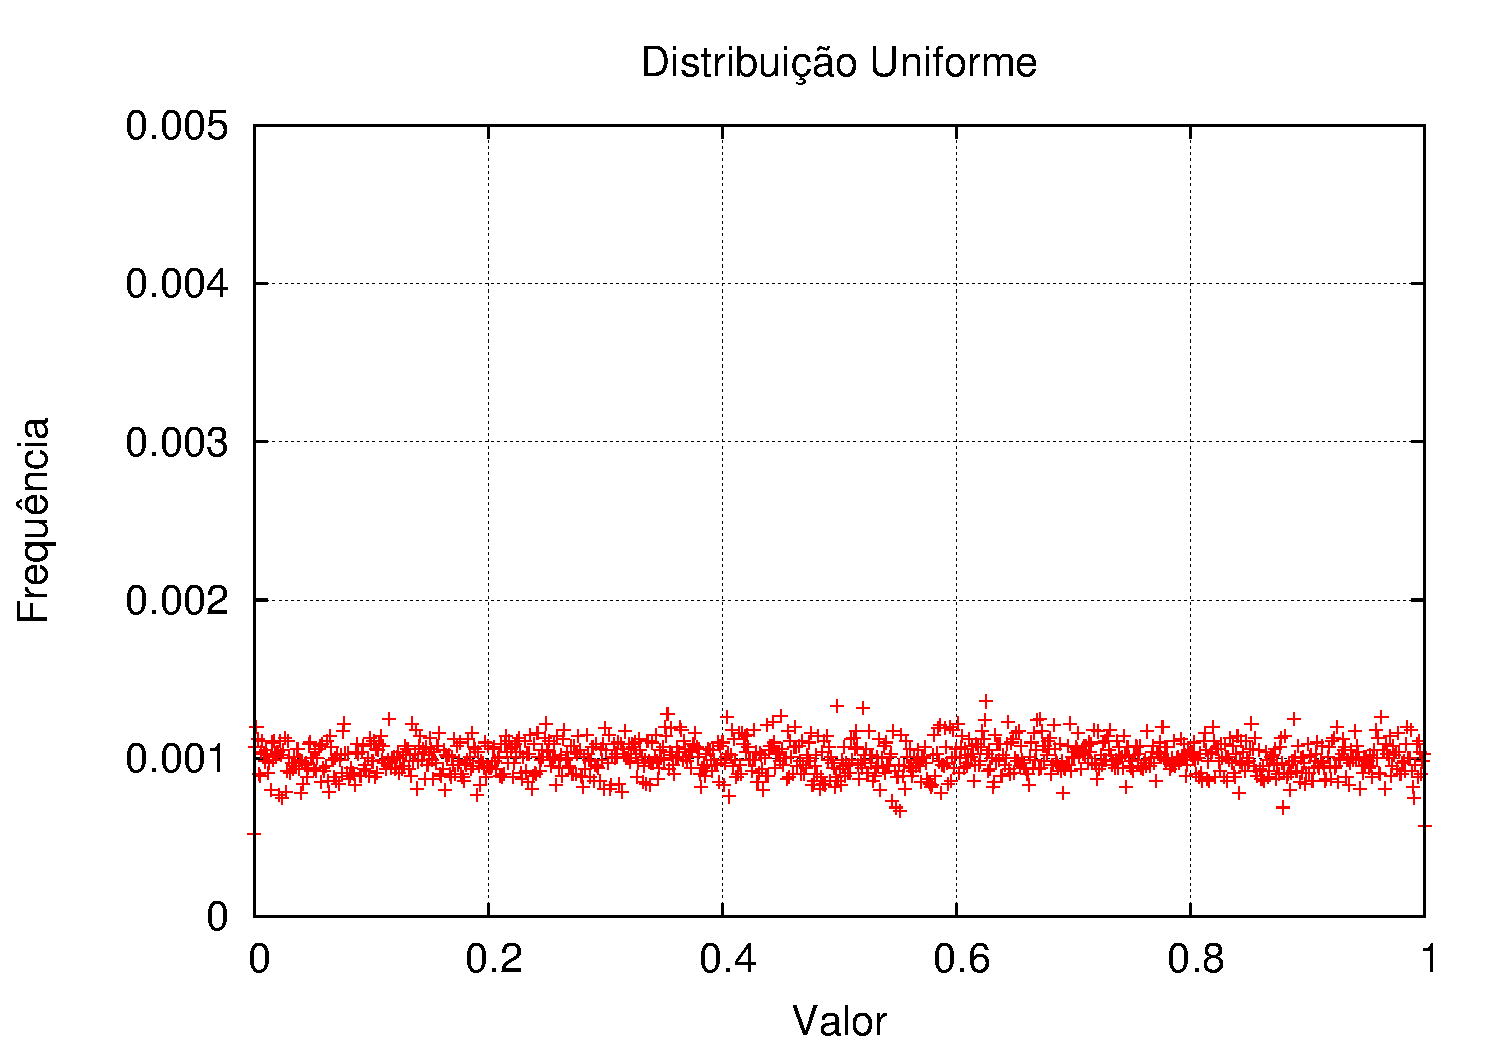
\includegraphics[width=0.48\textwidth]{figuras/DistribuicaoUniforme.pdf} \label{fig:uniforme}}
\subfigure[Distribuição Normal]{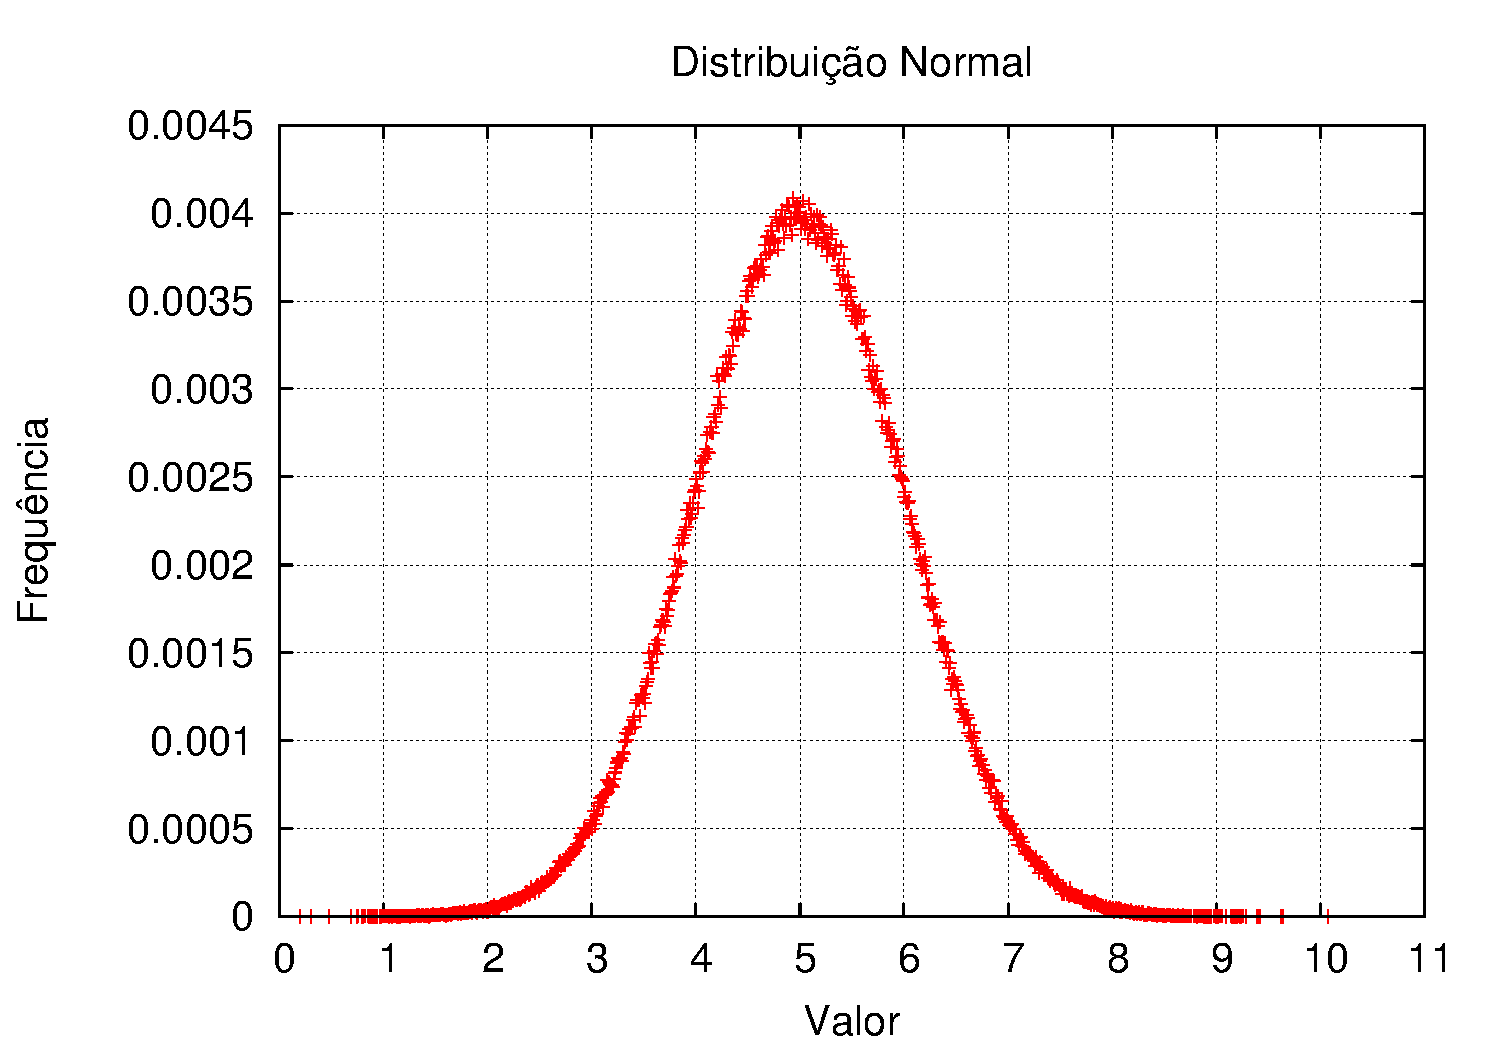
\includegraphics[width=0.48\textwidth]{figuras/DistribuicaoNormal.pdf} \label{fig:normal}}
% \subfigure[Distribuição Pareto]{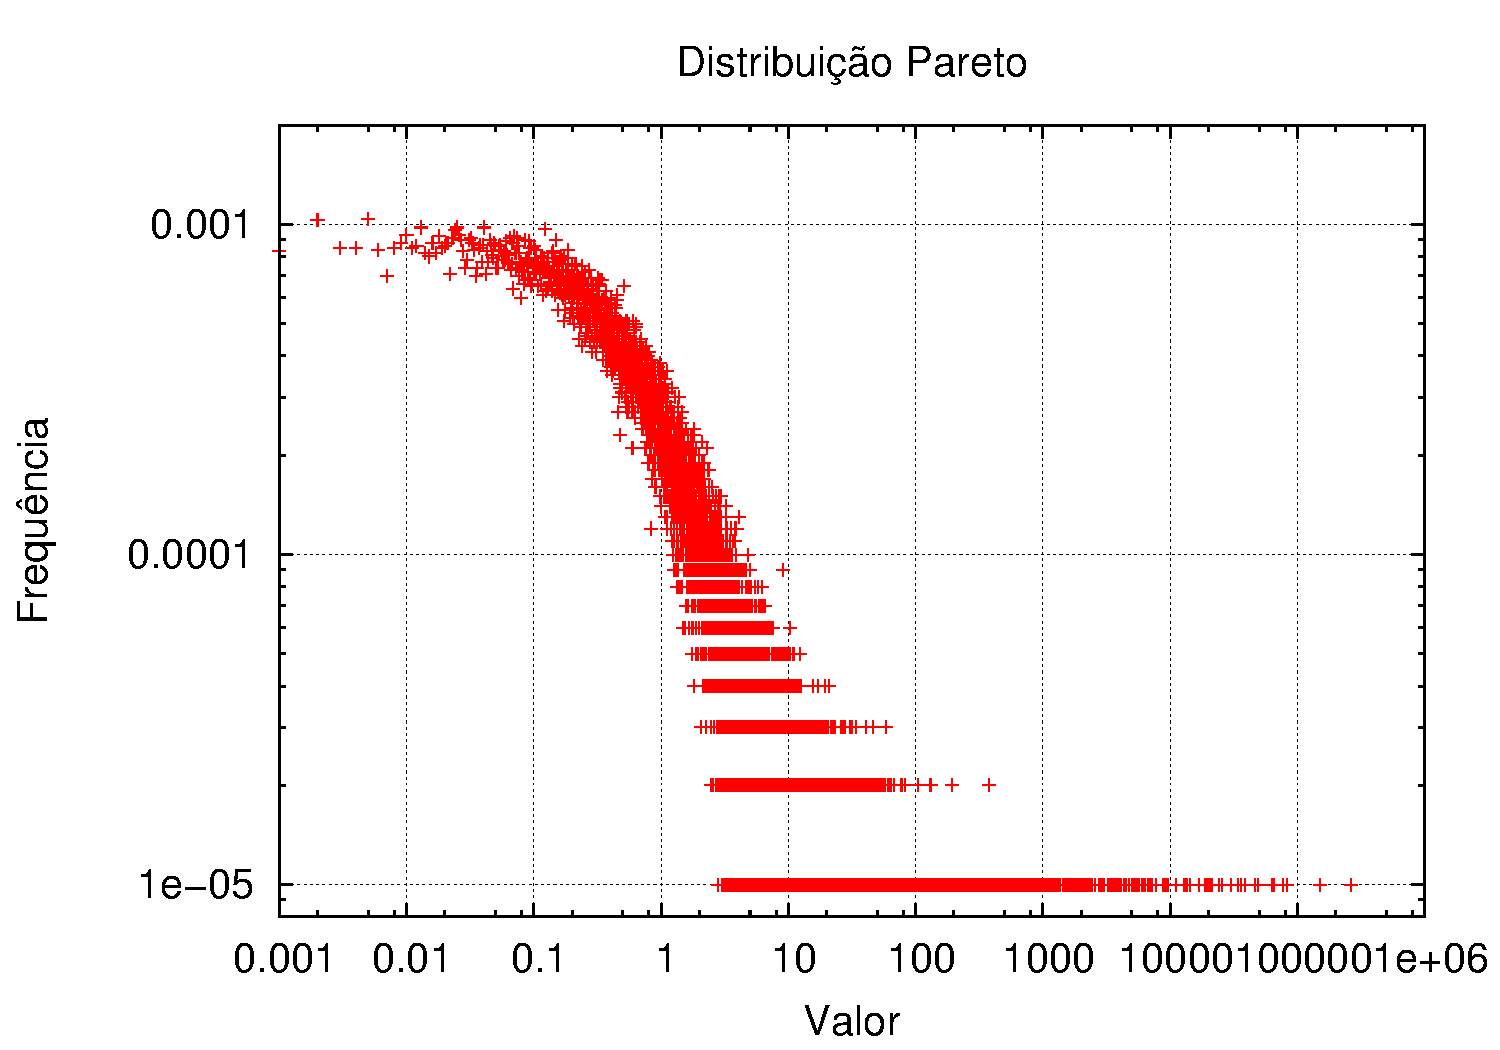
\includegraphics[width=0.48\textwidth]{figuras/DistribuicaoPareto.pdf} \label{fig:pareto}}
\caption{Distribuições dos dados gerados para ordenação}

\end{figure}


\section{Métricas de avaliação}

Os testes 


\subsection{Ordenação por Amostragem}

Os experimentos com o algoritmo Ordenação por Amostragem foram divididos em duas fases. A primeira fase consistiu na reprodução dos testes realizados no trabalho de referência, com o algoritmo implementado em Java, no ambiente Hadoop. A segunda fase dos experimentos consistiu em executar o algoritmo em cenários diferentes dos que já haviam sido apresentados. O objetivo de cada experimento era avaliar o algoritmo em situações diversas, confirmando sua escalabilidade e eficiência.

%Foram feitos três tipos de experimentos com o algoritmo, com alterações: (i) no número de arquivos, (ii) no número de máquinas e (iii) carga de dados. Em todos os casos utilizou-se a distribuição uniforme, similar à utilizada no trabalho de Pinhão (2011).

Os experimentos realizados nas duas fases podem ser divididos em três categorias, de acordo com as variações propostas: (i) no número de arquivos e (ii) no número de máquinas. 
O primeiro experimento manteve constante tanto o tamanho do arquivo a ser ordenado quanto o número de máquinas utilizadas na ordenação. 
O segundo experimento manteve constante o número de máquinas utilizadas e variou o tamanho do arquivo a ser ordenado. 
Já o terceiro experimento manteve constante o número de dados e alterou a quantidade de máquinas utilizadas. 

Na primeira fase, foram realizados os três experimentos, e em todos os casos utilizou-se a distribuição uniforme na geração dos dados, similar à utilizada no trabalho de Pinhão (2011). Os arquivos gerados continham entre $10^{6}$ (12MB) e  $10^{10}$ (120GB) chaves, e o número de máquinas utilizadas variou de 2 a 5.
Na segunda fase, cada um dos experimentos foi realizado com três conjuntos diferentes de dados.


Uma parte fundamental do algoritmo de Ordenação por Amostragem é a definição dos parâmetros de amostragem de chaves, para uma amostragem que resulte em partições balanceadas. Nos testes realizados, os parâmetros definidos foram o número máximo de amostras e o número de partições para cada caso.  O número máximo de amostras foi fixado em 10 mil, e o número de partições foi função do número de máquinas utilizadas e núcleos dos processadores: \mbox{$ Parti \text{\c{c}} \tilde{o}es = m\acute{a}quinas \times n\acute{u}cleos $}. Dessa forma, para as máquinas utilizadas, que contêm 2 núcleos, obtém-se: 4 partições para 2 máquinas; 6 para 3 máquinas; 8 para 4 máquinas; 10 para 5 máquinas.

A seguir são descritos os três tipos de testes realizados, especificando o número de máquinas utilizadas, o número de arquivos e o tamanho dos arquivos ordenados, assim como os objetivos de avaliação de cada teste.

\subsubsection{Testes de estabilidade}

\subsubsection{Variando o número de partições}

\subsubsection{Variando a distribuição dos dados} 

Os testes com número constante de máquinas e dados foram realizados em 4 máquinas, com arquivos de $10^{6}$ chaves. Foram feitos testes com 10 conjuntos de dados diferentes e, para cada conjunto, o algoritmo foi executado 10 vezes, com os parâmetros de balanceamento descritos anteriormente.  O objetivo foi avaliar a influência dos valores gerados aleatoriamente no desempenho do algoritmo. 


\subsubsection{Variando a quantidade de dados}
 
 Os testes variando a quantidade de dados também foram executados em 4 máquinas, com conjuntos de dados das três distribuições diferentes. Cada distribuição gerou aleatoriamente uma quantidade de dados entre $10^{6}$ e $10^{10}$. O algoritmo foi executado três vezes em cada conjunto com os parâmetros descritos anteriormente. O objetivo foi avaliar a complexidade do algoritmo quando o tamanho do conjunto de dados a ser ordenado aumenta.
 
\subsubsection{Variando a quantidade de máquinas}

Esses testes foram executados com tamanho constante do arquivo de entrada  ($10^{8}$ chaves) em quantidades de máquinas que variaram de 2 a 5. 
Para cada número de máquinas foram gerados conjuntos com as distribuições diferentes. O algoritmo foi executado três vezes para cada conjunto, com os parâmetros de balanceamento descritos anteriormente. O objetivo foi avaliar a escalabilidade do algoritmo, com diminuição do tempo de ordenação quando se aumenta o número de máquinas.


Os resultados dos testes com quantidade constante de máquinas e dados, variando a quantidade de dados e variando a quantidade de máquinas são apresentados e discutidos no Capítulo \ref{cap:resultados}.

\subsection{Validação dos resultados}

Para validar o resultado da ordenação realizada pelos algoritmos, foi desenvolvido um módulo para validação dos arquivos escritos, com função similar a do \textit{TeraValidade}. 
Essa aplicação deve ser executada após a ordenação completa, e verifica se alguma das chaves presentes no arquivo final está desordenada. O funcionamento é simples: o programa lê sequencialmente os arquivos ordenados e compara a chave atual com a anterior, e caso seja encontrado um valor fora de ordem, o programa escreve este valor no arquivo de saída. 
A execução de um programa de validação garante que o resultado da ordenação está correto, comprovando o funcionamento dos algoritmos desenvolvidos. 
Durante a realização dos testes, esse módulo era executado após a ordenação e confirmou que a execução estava correta em todos os casos testados.



\section{Ambiente de Desenvolvimento - OK}

O ambiente necessário ao desenvolvimento e execução do projeto foi fornecida pelo Laboratório de Redes e Sistemas (LABORES) do Departamento de Computação (DECOM) do Centro Federal de Educação Tecnológica de Minas Gerais. O LABORES possui um \textit{cluster} formado por cinco máquinas Dell Optiplex 380, que foram os recursos utilizados na realização dos testes de desempenho.

Cada máquina do \textit{cluster} apresenta as seguintes características:
\begin{packed_enum}
\item Processador Intel Core 2 Duo de 3.0 GHz
\item Disco rígido SATA de 500 GB 7200 RPM
\item Memória RAM de 4 GB
\item Placa de rede Gigabit Ethernet
\item Sistema operacional Ubuntu 10.04 32 bits %(kernel 2.6.\textbf{XX})
\item Sun Java JDK 1.6.0 19.0-b09 
\item Apache Hadoop 1.0.2
\end{packed_enum}


O próximo Capítulo apresenta os resultados coletados a partir da execução dos algoritmos no ambiente citado. 
			% Resultados
	%
% Documento: Resultados 
%

\chapter{Resultados}
\label{cap:resultados}

Neste capítulo são apresentados e analisados os resultados obtidos com a realização dos experimentos de ordenação no ambiente Hadoop.

A primeira parte dos experimentos consistiu em testes para conhecer o framework utilizado, o ambiente de execução e validar o funcionamento dos algoritmos de ordenação a serem comparados. A segunda parte dos experimentos iniciou-se após essa fase de reconhecimento, com a realização dos testes para avaliação de desempenho dos algoritmos Ordenação por Amostragem e Quicksort executados de acordo com o planejamento descrito anteriormente na Seção \ref{sec:experimentos}. 


%Esses experimentos foram  
%, e o reproduzir os resultados já encontrados no trabalho de referência: testes de ordenação com os \textit{benchmarks TeraSort} e \textit{Sort}, e com o algoritmo Ordenação por Amostragem em distribuição uniforme. 

A execução inicial de testes com os algoritmos distribuídos com o próprio ambiente Hadoop são fundamentais para a compreensão do funcionamento do ambiente de execução, incluindo a conexão entre as máquinas que compõem o \textit{cluster}.  
A importância desses testes consiste no fato de tais  aplicações serem conhecidas e consolidadas no ambiente Hadoop, e fornecerem exemplos de aplicações de ordenação desenvolvidas no modelo MapReduce.

O \textit{TeraSort} consiste de três algoritmos, que são responsáveis pela geração dos dados, ordenação e validação, conforme descrito na seção \ref{sec:benchmarks}.
Os testes com o \textit{TeraSort} foram feitos em duas máquinas. Foram gerados pelo \textit{TeraGen} dois arquivos contendo 50 mil linhas cada e o algoritmo foi executado 10 vezes.

O \textit{Sort} é um dos \textit{benchmarks}  de ordenação de dados mais conhecidos para Hadoop. Para os testes realizados com esse algoritmo foram utilizados dados gerados pelo algoritmo \textit{RandomWriter}. Para cada máquina do \textit{cluster}, foram escritos 10 arquivos de 1GB cada em formato binário, totalizando 10GB.

Os testes realizados inicialmente com os \textit{benchmarks} \textit{TeraSort} e \textit{Sort} permitiram um melhor entendimento sobre o funcionamento do \textit{framework} e dos algoritmos de ordenação nesse ambiente, que são objeto de estudo do presente trabalho. 

Os testes feitos com o algoritmo Ordenação por Amostragem tinham como objetivo reproduzir os
resultados encontrados no trabalho feito por Pinhão (2011), e gerar resultados 
que serão utilizados na comparação de desempenho dos dois algoritmos. 


Antes da execução dos experimentos de avaliação de desempenho, foram realizados diversos
testes de verificação com o objetivo de comprovar o funcionamento do algoritmo Quicksort em cenários variados,
com diferentes entradas, quantidade de dados e máquinas.
Os testes envolveram arquivos compostos de valores aleatórios, de valor único ou de dois valores,
e em todos os casos foi possível comprovar o correto funcionamento do algoritmo.
 



O resultado dos experimentos está separado de acordo com o tipo de teste realizado, com variação do número de partições,
da distribuição dos dados, da quantidade de dados ordenada e da quantidade de máquinas utilizadas. 


% --------------------------------------------------------
% ----------------- ESTABILIDADE -------------------------
% --------------------------------------------------------
\newpage
\section{Estabilidade do Sistema}

Os testes de estabilidade avaliam a variabilidade do tempo de resposta na execução do algoritmo, que é diretamente afetado pelo tamanho das partições formadas. 

\begin{defaultFigure}{0.75\textwidth}{graficos/EstabilidadeTempo.pdf}
{Gráfico do tempo para ordenação de conjuntos de 10$^8$ dados em 5 máquinas}
\label{fig:EstabilidadeTempo}
\end{defaultFigure}

O tamanho das partições dos dois algoritmos separados, em escalas diferentes.
\begin{defaultFigure}{0.75\textwidth}{graficos/EstabilidadeParticoes1.pdf}
{Partições obtidas na ordenação de conjuntos de 10$^8$ dados em 5 máquinas}
\label{fig:EstabilidadeParticoes}
\end{defaultFigure}


% --------------------------------------------------------
% ----------------- PARTIÇÕES ----------------------------
% --------------------------------------------------------
\newpage
\section{Variando o Número de Partições}

<INCLUIR DESCRIÇÃO GRÁFICO TEMPO>
 
\begin{defaultFigure}{0.75\textwidth}{graficos/ParticoesTempo.pdf}
{Gráfico do tempo para ordenação de conjuntos de 10$^8$ dados em 5 máquinas com diferentes números
de partições}
\label{fig:ParticoesTempo}
\end{defaultFigure}

% --------------------------------------------------------
% ----------------- DISTRIBUIÇÃO -------------------------
% --------------------------------------------------------
\newpage
\section{Variando a Distribuição de Dados}

<TEXTO> 

<DESCRIÇÃO GRÁFICO TEMPO>
\begin{defaultFigure}{0.75\textwidth}{graficos/DistribuicaoTempo.pdf}
{Gráfico dos tempos médios para ordenação de 10$^8$ dados em 5 máquinas}
\label{fig:DadosTempos}
\end{defaultFigure}

<TABELA TEMPO>

<DESCRIÇÃO GRÁFICO PARTIÇÕES>
% \begin{defaultFigure}{0.75\textwidth}{graficos/DistribuicaoTempo.pdf}
% {Gráfico dos tempos médios para ordenação de 10$^8$ dados em 5 máquinas}
% \label{fig:DadosTempos}
% \end{defaultFigure}

<TABELA PARTIÇÕES>

% --------------------------------------------------------
% -------------------- DADOS -----------------------------
% --------------------------------------------------------

\newpage
\section{Variando a Quantidade de Dados}

Os testes variando a quantidade de dados buscavam avaliar a complexidade dos dois algoritmos,
observando seu comportamento com o aumento na entrada de dados. Para esse teste, foram feitas
execuções com dados uniformes, com quantidade variando de 10$^6$ a 10$^{10}$. 
O algoritmo Quicksort foi executado com 2 partições, e Samplesort manteve a fórmula anteriormente
usada: partições = máquinas x núcleos. As ordenações
foram feitas em cinco máquinas, e o teste foi repetido 5 vezes para cada quantidade de
dados. 
A seguir são apresentados os tempos de ordenação total e relativo a cada conjunto de 10$^6$ dados,
que incluem a média dos tempos para as 5 execuções.


A Figura \ref{fig:DadosTempos} apresenta o tempo médio de ordenação de cada conjunto. O gráfico
apresenta os eixos x e y em escala logarítmica para melhor visualização. Os resultados mostram que
o tempo médio do Quicksort foi ligeiramente menor com o conjunto de 10$^6$ dados, mas nos demais
casos se manteve acima do tempo médio do Samplesort. Além disso, quanto maior o
arquivo, maior foi a diferença entre os tempos. 

\begin{defaultFigure}{0.75\textwidth}{graficos/DadosTempo.pdf}
{Gráfico dos tempos médios para ordenação de 10$^6$ a 10$^{10}$ dados em 5 máquinas}
\label{fig:DadosTempos}
\end{defaultFigure}
 

<INCLUIR DESCRIÇÃO DA TABELA>
\begin{defaultTable}{| B R{5}}
{
\multirow{2}{*}{Dados} & \multicolumn{2}{T}{Tempo (s) Quicksort}  & \multicolumn{2}{T}{Tempo (s)
Samplesort}  \\\cline{2-5}
\rowstyle{\bfseries} 
			&	Média	&	COV		&	Média	&	COV		\\ \hline \hline
$10^6$		&	18		&	0.001	&	20		&	0.004	\\ \hline
$10^7$		&	34		&	0.025	&	30		&	0.028	\\ \hline
$10^8$		&	212		&	0.017	&	144		&	0.010	\\ \hline
$10^9$		&	2246	&	0.036	&	1356	&	0.027	\\ \hline
$10^{10}$	&	30246	&	0.085	&	14816	&	0.005	\\ \hline


}
{Tempos estatísticos para ordenação de diferentes quantidades de dados em 5 máquinas}
\label{tab:DadosTempo}
\end{defaultTable}


Com a finalidade de dimensionar o \textit{overhead} do algoritmo, isto é, a sobrecarga ou custo
adicional de comunicação entre os processadores mestre e escravos, assim como sua escalabilidade em
relação ao número de dados, foi calculado o tempo médio relativo de ordenação para cada conjunto de
10$^6$ dados. 
 
<INLCUIR DESCRIÇÃO GRÁFICO MEGADADOS>
 
\begin{defaultFigure}{0.75\textwidth}{graficos/DadosMegaDados.pdf}
{Gráfico do tempo médio relativo para ordenação de conjuntos de 10$^6$ dados em 5 máquinas}
\label{fig:DadosMegaDados}
\end{defaultFigure}
 
 
% DESCRIÇÃO GRÁFICO COMPLEXIDADE
% 
<INCLUIR GRÁFICO COMPLEXIDADE>
% 
% \newpage


% --------------------------------------------------------
% -------------------- MÁQUINAS --------------------------
% --------------------------------------------------------
\newpage
\section{Variando a Quantidade de Máquinas}

Os testes variando a quantidade de máquinas foram realizados para avaliar a escalabilidade do
algoritmo, de forma a medir o ganho de tempo obtido com o aumento do número de máquinas
utilizadas na ordenação. Para tal, cada algoritmo foi executado cinco vezes e foi medido o tempo
gasto na ordenação. 
Além do tempo gasto em cada execução, foram calculados também o \textit{speedup}
e a eficiência de cada algoritmo. Cada teste foi realizado com um conjunto de 10$^8$
chaves uniformes, que foram ordenadas por grupos de 2, 3, 4 e 5 máquinas.

A Figura \ref{fig:MaquinasTempos} representa graficamente a variação do tempo à medida que o número
de máquinas aumenta. Como se pode observar, a variação, representada pela inclinação da curva é
similar para os dois algoritmos, mantendo uma queda gradativa no tempo de execução com o aumento
do número de máquinas. Ainda pode-se observar que a diminuição do tempo não é linear, não
ocorre na mesma proporção que o aumento no número de máquinas. 


\begin{defaultFigure}{0.75\textwidth}{graficos/MaquinasTempo.pdf}
{Gráfico dos tempos médios para ordenação de 10$^8$ dados em 2 a 5 máquinas}
\label{fig:MaquinasTempos}
\end{defaultFigure}

As Tabelas \ref{tab:MaquinasTempoS} e \ref{tab:MaquinasTempoQ} apresentam os tempos médios, em
segundos,
necessários para as ordenações de $10^8$ elementos em diferentes quantidade de máquinas, com os
algoritmos Quicksort e Samplesort, respectivamente. 

O tempo médio para a execução em duas máquinas do algoritmo Samplesort foi de aproximadamente 6
minutos, do algoritmo Quicksort foi perto de 7 minutos. Em três máquinas o algoritmo Samplesort
gastou cerca de 4 minutos para concluir a ordenação, 36\% menos que o Quicksort, que precisou
de pouco mais de 5 minutos.
Com quatro máquinas os tempos de execução para Samplesort e Quicksort foram de aproximadamente 3 e 4
minutos, respectivamente.
Em cinco máquinas a ordenação foi realizada em aproximadamente 4 minutos
com Quicksort e 2 minutos com Samplesort. De forma geral, a avaliação dos resultados mostra que
para cada acréscimo de uma máquina houve uma diminuição de 1 minuto no tempo de execução do
algoritmo.

\begin{defaultTable}{| B R{6}}
{
\multirow{2}{*}{Máquinas} & \multicolumn{6}{T}{Tempo (s) Samplesort}  \\\cline{2-7}
\rowstyle{\bfseries} 
		&	Menor	&	Maior	&	Média	&	Mediana	&	Desvio Padrão	& 	COV	\\ \hline \hline
2		&	328		&	338	&	334	&	335	&	3,344			&	0,010	\\ \hline
3		&	225		&	230	&	227	&	227	&	1,735			&	0,008	\\ \hline
4		&	175		&	182	&	178	&	177	&	2,518			&	0,014	\\
\hline
5		&	139		&	144	&	142	&	142	&	1,864			&	0,013	\\
\hline
}
{Tempos estatísticos para ordenação com Samplesort de $10^8$ chaves em diferentes quantidades de
máquinas}
\label{tab:MaquinasTempoS}
\end{defaultTable}

\begin{defaultTable}{| B R{6}}
{
\multirow{2}{*}{Máquinas} & \multicolumn{6}{T}{Tempo (s) Quicksort}  \\\cline{2-7}
\rowstyle{\bfseries} 
	&	Menor	&	Maior	&	Média	&	Mediana	&	Desvio Padrão	&	COV	\\ \hline \hline
2	&	399	&	415	&	406	&	404	&	5,450			&	0,013	\\ \hline
3	&	291	&	320	&	309	&	312	&	9,724			&	0,031	\\ \hline
4	&	247	&	267	&	256	&	256	&	7,101			&	0,028	\\ \hline
5	&	215	&	233	&	224	&	220	&	6,938			&	0,031	\\ \hline
}
{Tempos estatísticos para ordenação com Quicksort de $10^8$ chaves em diferentes quantidades de máquinas}
\label{tab:MaquinasTempoQ}
\end{defaultTable}

O tempo médio de execução do algoritmo Quicksort em cinco máquinas foi cerca de 45\% menor que o
tempo médio obtido em duas máquinas. 
Para o Samplesort o percentual reduzido é ainda maior: em cinco máquinas reduz-se 57\% o tempo
necessário para a execução em duas máquinas. 

Em todos os casos, o coeficiente de variação calculado foi menor que 0,03, o que indica
tempos de execução bastante homogêneos para os dois algoritmos. 




A fim de avaliar o desempenho do algoritmo nas diferentes configurações de máquinas foram calculadas
as métricas \textit{speedup}
e eficiência.

Como foi descrito na Seção \ref{sec:computacaoparalela}, o \textit{speedup} indica quão mais rápida
é a aplicação paralela comparada à aplicação sequencial. Já a eficiência  indica a taxa de
utilização de cada processador. Ela é  excelente quando é 100\%, indicando que os processadores tem
utilização total.
Nesse trabalho o algoritmo foi implementado apenas em paralelo, assim, considera-se para fins de
comparação a execução em quatro processadores (duas máquinas), ao invés da execução sequencial. As
fórmulas
foram adaptadas para verificar a melhora de desempenho e eficiência obtidas a partir de duas
máquinas: 
\[ S = \frac{T_{4 \quad processadores}}{T_{paralelo}}  
\quad\mbox{e}\quad
 E = \frac{S_{real}}{S_{ideal}}\]

Os tempos descritos nas Tabelas \ref{tab:MaquinasTempoS} e \ref{tab:MaquinasTempoQ} foram
utilizados no cálculo do \textit{speedup} e, consequentemente, da eficiência.
A Tabela \ref{tab:MaquinasSpeedup} mosta os valores do \textit{speedup} real calculado e o valor
ideal para comparação. 
Considera-se que a execução com quatro processadores é o valor de referência, e assim
o \textit{speedup} real é igual ao ideal. 
Observa-se que à medida que aumenta o número de processadores o \textit{speedup} real se afasta do
\textit{speedup} ideal. 
A variação do \textit{speedup} já era um comportamento esperado, uma vez que paralelizações em geral
introduzem sobrecargas para realizar o balanceamento e a comunicação entre os processos.

\begin{defaultTable}{|N{25mm}|C{24mm}|C{24mm}|C{12mm}| }
{
\multirow{2}{*}{Processadores} & \multicolumn{2}{T}{Speedup Real} & \multirow{2}{*}{Ideal} \\ \cline{2-3}
\rowstyle{\bfseries} 
	&	Samplesort  &	Quicksort &	\\ \hline \hline
4	&	1			&	1		&	1	\\ \hline
6	&	1,457		&	1,312	&	1,5	\\ \hline
8	&	1,875		&	1,586	&	2	\\ \hline
10	&	2,348		&	1,813	&	2,5	\\ \hline
}
{Resultados do \textit{speedup} para execuções de 4 a 10 processadores}
\label{tab:MaquinasSpeedup}
\end{defaultTable}


A Figura \ref{fig:MaquinasSpeedup} apresenta a curva do \textit{speedup} real dos algoritmos
Quicksort e Samplesort à medida que o número de processadores aumenta, além  da curva de
\textit{speedup} ideal para comparação. 
Como se pode ver, inicialmente todos os valores de \textit{speedup} são iguais mas, com o aumento no número de processadores, a curva representando o valor do \textit{speedup} real se afasta da curva
do \textit{speedup} ideal, fato que ocorre com maior acentuação no algoritmo Quicksort.


\begin{defaultFigure}{0.75\textwidth}{graficos/MaquinasSpeedup.pdf}
{Gráfico do \textit{speedup} para ordenação de 10$^8$ dados em em 2 a 5 máquinas}
\label{fig:MaquinasSpeedup}
\end{defaultFigure}

A Tabela \ref{tab:MaquinasEficiencia} apresenta os valores de eficiência calculados para as
diferentes quantidades de processadores utilizados na ordenação. Observa-se que, conforme aumenta a
quantidade de processadores, o valor da eficiência decresce, mostrando que, com maior número de
processadores, a taxa de utilização é menor. Além disso, observa-se que a eficiência
do algoritmo Samplesort é maior que a eficiência do Quicksort o que indica uma melhor escalabilidade
do algoritmo Samplesort. 

\begin{defaultTable}{|N{25mm}|C{24mm}|C{24mm}| }
{
\multirow{2}{*}{Processadores} & \multicolumn{2}{T}{Eficiência (\%)} \\
\cline{2-3}
\rowstyle{\bfseries} 
	&	Samplesort  &	Quicksort 	\\ \hline \hline
4	&100				&	100			\\ \hline
6	&97,12			&	91,39		\\ \hline
8	&93,97			&	80,82		\\ \hline
10	&94,70			&	74,10		\\ \hline
}
{Resultados da \textit{eficiência} para execuções de 4 a 10 processadores}
\label{tab:MaquinasEficiencia}
\end{defaultTable}



A Figura \ref{fig:MaquinasEficiencia} representa graficamente a eficiência em diferentes números de
processadores. Nela observa-se que, à medida que o número de processadores aumenta o percentual da
eficiência diminui, o que ocorre mais acentuadamente no algoritmo Quicksort. 

\begin{defaultFigure}{0.75\textwidth}{graficos/MaquinasEficiencia.pdf}
{Gráfico da eficiência para ordenação de 10$^8$ dados em em 2 a 5 máquinas}
\label{fig:MaquinasEficiencia}
\end{defaultFigure}

\section{Considerações Finais}
			% Resultados
	%
% Documento: Conclusões
%

\chapter{Conclusões}
\label{cap:conclusoes}


\section{Trabalhos Futuros}
\label{sec:trabalhosFuturos}

			% Conclusões

% elementos pós textuais
	%
% Documento: Referências Bibliográficas
%

\bibliographystyle{abnt-alf}
\bibliography{./bibliografia}	% geracao automatica das referencias a partir do arquivo refbase.bib
		% Referências
	%\include{./elementos-pos-textuais/glossario} 		% Glossário
	%%
% Documento: Apêndice
%

\apendice
\chapter{Nome do apêndice}
\label{chap:apendicex}

Inserir seu texto aqui...

\chapter{Nome do apêndice}
\label{chap:apendicey}

Inserir seu texto aqui...
 		% Apêndices
	%%
% Documento: Anexos
%

\anexo
\chapter{Nome do anexo}
\label{chap:anexox}

Inserir seu texto aqui...

\chapter{Nome do anexo}
\label{chap:anexoy}

Inserir seu texto aqui...
			% Anexos
	%\include{./elementos-pos-textuais/indices}			% Índices

\end{document}
